%----------------------------------------------------------------
%
%  File    :  survey.tex
%
%  Author  :  Mirza Kabiljagic, Stefan Rajinovic, Aleksandar Stojicic
%             Inti Gabriel Mendoza Estrada
%
%  Created :  24 Mar 2010
%
%  Changed :  04 Mar 2019
%
%----------------------------------------------------------------


\documentclass[11pt,onecolumn,twoside]{report}
\usepackage{amsmath}
\usepackage{nccmath}


\usepackage[
  a4paper,
  twoside,
  top=5mm,                % top margin
  bottom=7mm,             % bottom margin
  inner=20mm,             % inner margin (next to binding)
  outer=20mm,             % outer margin (opposite binding)
  bindingoffset=10mm,     % on binding side
  includeheadfoot,        % include head(er) and foot(er)
  headheight=10mm,        % height of header
  headsep=15mm,           % sep between header and text body
  footskip=15mm,          % sep between body and baseline of footer
  footnotesep = 10mm plus 2mm minus 0mm  % bottom of body to top of footnote
]{geometry}
% A4 paper is w=210m, h=297mm



\newcommand{\fullh}{24cm}         % height of figures for 1 per page
\newcommand{\halfh}{9.5cm}        % height of figures for 2 per page
\newcommand{\thirdh}{6cm}         % height of figures for 3 per page


\setlength{\parindent}{1em}       % less indentation
\setlength{\parskip}{5pt plus 1pt minus 1pt}  % space before a paragraph


% \tolerance is set by LaTeX to 200
% \sloppy sets \tolerance = 9999
% which allows LaTeX more tolerance in adding word spacing

% \sloppy
% \fussy
% \tolerance = 1000

\tolerance=400 
% makes some lines with lots of white space, but      
% tends to prevent words from sticking out in the margin



\setcounter{tocdepth}{3}        % lowest section level entered in ToC
\setcounter{secnumdepth}{3}     % lowest section level still numbered




\usepackage[T1]{fontenc}        % 8-bit output chars (must be before inputenx)
\usepackage[utf8]{inputenx}     % input char encoding

\usepackage[english,austrian,british]{babel}

\usepackage{newtxtext}          % newer times fonts
\usepackage{newtxmath}

\usepackage{relsize}            % relative font sizes \smaller \larger
\usepackage{float}              % H for float placement
\usepackage{setspace}           % line spacing

\usepackage{textcomp}           % symbols such as \texttimes and \texteuro
\usepackage{latexsym}
\usepackage{fontawesome}        % fontawesome symbols

\usepackage{siunitx}            % prettier number formatting
\sisetup{%
  group-separator={,},
}
\usepackage[super]{nth}         % 1st, 2nd, 3rd, etc.

\usepackage{xspace}
\usepackage{xstring}            % string manipulation macros
\usepackage{xparse}             % commands with optional arguments
\usepackage{etoolbox}           % for \newrobustcmd
\usepackage{makecmds}           % for \makecommand
\usepackage{calc}               % for math calculations

\usepackage[svgnames,table,xcdraw]{xcolor}
\definecolor{darkgreen}{rgb}{0.0,0.2,0.0}
\definecolor{darkblue}{rgb}{0.0,0.0,0.2}
\definecolor{darkred}{rgb}{0.2,0.0,0.0}
\definecolor{verylightgrey}{gray}{0.95}
\definecolor{lightgrey}{gray}{0.9}
\definecolor{grey}{gray}{0.7}
\definecolor{black}{gray}{0.0}


\usepackage{longtable}
\usepackage{multirow}
\usepackage{tabularx}

\usepackage{verbdef}            % define robust verb strings
\usepackage{verbatim}
\usepackage{comment}



% better lists
\usepackage{enumitem}

\setlist{
  topsep=0pt,
  partopsep=0pt,
  parsep=0.6ex,
  itemsep=1.2ex,
  left=\parindent .. 2\parindent,    % bullet .. start ot text
}

\setlist[description]{
  style=sameline,
}




\usepackage{listings}                 % for listings of source code

\makeatletter
\newlength{\numwidth}%
\setlength{\numwidth}{\widthof{\normalfont{\lst@numberstyle{99}}}}% Up to 2-digit (99) line numbers
\def\lst@PlaceNumber{%
  \makebox[\numwidth+1em][l]{%
    \makebox[\numwidth][r]{\normalfont\lst@numberstyle{\thelstnumber}}%
  }%
}
\makeatother

% lstset strategy: define defaults here for
% all non-floating listings
% floated listings override these settings later

\lstset{                              % set parameters for listings
  floatplacement=tp,                  % default float placement
  numberbychapter,
  inputencoding=utf8,
  language=,                          % empty = plain text
  basicstyle=\small\ttfamily,
  tabsize=2,
  xleftmargin=2\parindent,
  xrightmargin=2\parindent,
  frame=none,
  framexleftmargin=0mm,
  rulesepcolor=\color{verylightgrey},
  numbers=none,
  numberstyle=\scriptsize,
  numbersep=2ex,
  breaklines,
  showtabs=false,
  showspaces=false,
  showstringspaces=false,
  keywordstyle=\color{black},
  commentstyle=\color{SteelBlue},
  identifierstyle=,
  stringstyle=,
  captionpos=b,
  abovecaptionskip=\abovecaptionskip,
  belowcaptionskip=\belowcaptionskip,
  extendedchars=true,
  literate=%
    {©}{{\textcopyright}}1
    {€}{{\texteuro}}1
    {Ö}{{\"O}}1
    {Ä}{{\"A}}1
    {Ü}{{\"U}}1
    {ß}{{\ss}}1
    {ö}{{\"o}}1
    {ä}{{\"a}}1
    {ü}{{\"u}}1,       % map some utf8 chars for listings
}


\lstdefinelanguage{biblatex}   % based on biblatex v 2.7a from 2013-07-14
{
  keywords={%
    @article,@book,@mvbook,@inbook,@bookinbook,@suppbook,%
    @booklet,@collection,@mvcollection,@incollection,@suppcollection,%
    @manual,@misc,@online,@patent,@periodical,@suppperiodical,%
    @proceedings,@mvproceedings,@inproceedings,@reference,@mvreference,%
    @inreference,@report,@set,@thesis,@unpublished,@xdata,%
    @conference,@electronic,@mastersthesis,@phdthesis,@techreport,@www,%
    @artwork,@audio,@bibnote,@commentary,@image,@jurisdiction,@legislation,%
    @legal,@letter,@movie,@music,@performance,@review,@software,%
    @standard,@video%
  },
  sensitive=false,
  comment=[l][\itshape]{@comment},
  morecomment=[l]{\%},
}

\lstdefinelanguage{CSS}
{
  alsoletter={-},
  morekeywords={%
  color,background,background-color,margin,padding,font,
  font-family,weight,%
  display,position,top,left,right,bottom,list,%
  style,border,size,white,space,min,width%
  },
  sensitive=false,
  morecomment=[l]{//},
  morecomment=[s]{/*}{*/},
  morestring=[b]",
}





\usepackage[compact,nobottomtitles,pagestyles,explicit]{titlesec}
% when using explicit, must explicitly include #1 for titlename

% nobottomtitles
% move section headings close to page bottom to next page
\renewcommand{\bottomtitlespace}{2cm}

% \chaptermark sets the value of \chaptertitle for later
% \@chapapp is defined as \chaptername outside the appendix,
% and as \appendixname within the appendix.
\makeatletter
\titleformat{\chapter}
[display]                                            % shape
{\chaptermark{\thechapter~~#1}\sffamily\bfseries}    % format
{\huge\@chapapp\ \thechapter}                        % label
{4ex}                                                % sep
{\Huge#1}                                            % before-code
\makeatother

\titleformat{name=\chapter,numberless}
[block]                                              % shape
{\chaptermark{#1}\sffamily\bfseries}                 % format
{}                                                   % label
{0ex}                                                % sep
{\Huge#1}                                            % before-code

\titleformat{\section}
{\normalfont\Large\sffamily\bfseries}{\thesection}{0.8em}{#1}

\titleformat{\subsection}
{\normalfont\large\sffamily\bfseries}{\thesubsection}{0.8em}{#1}

\titleformat{\subsubsection}
{\normalfont\normalsize\sffamily\bfseries}{\thesubsubsection}{0.8em}{#1}

\titleformat{\paragraph}[runin]
{\normalfont\normalsize\sffamily\bfseries}{\theparagraph}{0.8em}{#1}

\titleformat{\subparagraph}[runin]
{\normalfont\normalsize\sffamily\bfseries}{\thesubparagraph}{0.8em}{#1}


% vertical spacing before and after section titles
\titlespacing*{\section}
{0pt}{3.5ex plus 0.5ex minus 0.5ex}{0ex plus 0ex minus 0.2ex}

\titlespacing*{\subsection}
{0pt}{2.5ex plus 0.5ex minus 0.5ex}{0ex plus 0ex minus 0.2ex}

\titlespacing*{\subsubsection}
{0pt}{2ex plus 0.5ex minus 0.5ex}{0ex plus 0ex minus 0.2ex}


% define page headings how I want them

\newpagestyle{main}[\small]{
% \addtolength\headheight{6.7pt}
% \headrule
\sethead%
[{\parbox[t]{0.3\textwidth}%                    % even left
  {\sffamily\thepage}}]
[]%                                             % even centre
[{\parbox[t]{0.6\textwidth}%                    % even right
  {\raggedleft\sffamily\chaptertitle}}]
{{\parbox[t]{0.6\textwidth}%                    % odd left
  {\sffamily\sectiontitle}}}%
{}%                                             % odd centre
{{\parbox[t]{0.3\textwidth}%                    % odd right
  {\raggedleft\sffamily\thepage}}}
}



\usepackage{titletoc}

% Add extra per-chapter space to LoL to mimic LoF and LoT
% (requires package etoolbox)
\makeatletter
\patchcmd{\@chapter}% <cmd>
  {\addtocontents}% <search>
  {\addtocontents{lol}{\protect\addvspace{10\p@}}% add per-chapter space
   \addtocontents}% <replace>
  {}{}% <success><failure>
\makeatother

% Configure LoL to mimic LoF and LoT
\contentsuse{lstlisting}{lol}
\titlecontents{lstlisting}
  [3.8em]                      % left indent
  {\addvspace{1.5mm}}          % above-code per entry
  {\contentslabel{2.3em}}      % format for numbered entry
  {\hspace*{-2.3em}}           % format for unnumbered entry
  {\titlerule*[2.7mm]{.} \contentspage}  % dots and page num per entry
  []                           % below-code per entry

%\renewcommand{\lstlistlistingname}{List of Listings}





% sensible settings for floats

\setlength{\textfloatsep}{9mm plus 2mm minus 2mm}
\setlength{\floatsep}{9mm plus 2mm minus 2mm}
\setlength{\intextsep}{9mm plus 2mm minus 2mm}

\setlength{\dbltextfloatsep}{9mm plus 2mm minus 2mm}
\setlength{\dblfloatsep}{9mm plus 2mm minus 2mm}

\setlength{\abovecaptionskip}{4mm plus 2mm minus 1mm}
\setlength{\belowcaptionskip}{0mm}

% See http://www-rohan.sdsu.edu/~aty/bibliog/latex/floats.html
% See https://robjhyndman.com/hyndsight/latex-floats/

\setcounter{topnumber}{2}               % max num floats at top of page
\setcounter{dbltopnumber}{2}            % max num floats on 2col page
\setcounter{bottomnumber}{2}            % max num floats at bottom of page
\setcounter{totalnumber}{4}             % max num floats on a page

\renewcommand{\topfraction}{0.8}        % max fraction of floats at top
\renewcommand{\dbltopfraction}{0.9}     % max fraction of floats at top 2col
\renewcommand{\bottomfraction}{0.8}     % max fraction of floats at bottom
\renewcommand{\textfraction}{0.2}       % min fraction of text

% only for entirely float pages:
\renewcommand{\floatpagefraction}{0.7}      % min page fraction having floats
\renewcommand{\dblfloatpagefraction}{0.7}   % min 2col page fraction having floats


% \usepackage[section,above,below]{placeins}  % keep floats to their own section




% use caption and subfig (caption2 and subfigure are now obsolete)

\usepackage[
  position=bottom,
  margin=1cm,
  font=small,
  labelfont={bf,sf},
  format=hang,
  indention=0mm,
]{caption,subfig}

\captionsetup[subfigure]{
  margin=0pt,
  parskip=0pt,
  hangindent=0pt,
  indention=0pt,
  singlelinecheck=true,
  farskip=4mm,            % skip above subfig (assuming captions at bottom)
  captionskip=2mm,        % skip between subfig and subcaption
}


\usepackage[hyphens,obeyspaces]{url}
\def\UrlFont{\smaller\ttfamily}





\usepackage[short]{datetime}   % load datetime *after* babel, requires fmtcount
% \newdateformat{britdate}{%
% \ordinaldate{\THEDAY} \,\monthname[\THEMONTH] \THEYEAR
% }
\newdateformat{unixdate}{%
\twodigit{\THEDAY}~\shortmonthname[\THEMONTH]~\THEYEAR
}



\usepackage[
  autostyle=true,          % adapt quote style to current language
  english=british,         % british english as default
  threshold=1,             % set block quotations >1 line in display mode
  maxlevel=4,              % max nesting level
]{csquotes}

\usepackage[
  indentfirst=false,
  vskip=0pt,               % by default would be \topsep + \partopsep.
]{quoting}

% tell csquotes to use quoting environment
% for \displayquote and \blockquote
\SetBlockEnvironment{quoting}

% if cite is issued by a csquote command
\renewcommand{\mkcitation}[1]{\space#1}

% I prefer double quotes as outer
\DeclareQuoteStyle{keithbritish}%  [variant]{style}
  {\textquotedblleft}%                      opening outer mark
  {\textquotedblright}%                     closing outer mark
  [0.05em]%
  {\textquoteleft}%                         opening inner mark
  {\textquoteright}%                        closing inner mark

\ExecuteQuoteOptions{style=keithbritish}





\usepackage[
  backend=biber,
  style=ext-authoryear,        % defined in biblatex-ext package
  sorting=nyt,
  useprefix,                   % van and von are part of second name
  mergedate=false,             % only for authoryear style
  dashed=false,                % only for authoryear style
  abbreviate=false,
  maxcitenames=2,              % if > 2 authors,
  mincitenames=1,              % use first 1 then et al
  maxbibnames=99,              % if > 99 authors,
  minbibnames=6,               % use first 6 then et al
  uniquelist=minyear,
  uniquename=init,
  hyperref=true,
  backref=true,
  backrefstyle=two,
  sortlocale=en,
]{biblatex}


% set for csquotes, but \autocite only available
% after biblatex is loaded
\SetCiteCommand{\autocite}    % or maybe \parencite

% more space between entries in bib
\setlength\bibitemsep{1.5\itemsep}

% kandrews: replace round brackets with square brackets in citations
\DeclareOuterCiteDelims{parencite}{\bibopenbracket}{\bibclosebracket}
\DeclareInnerCiteDelims{textcite}{\bibopenbracket}{\bibclosebracket}

% kandrews: replace round brackets with square brackets in bibliography
% biblabeldate is a biblatex-ext feature
\DeclareFieldFormat{biblabeldate}{\mkbibbrackets{#1}}


% remove URL: from in front of URLs
\DeclareFieldFormat{url}{\url{#1}}
\DeclareFieldFormat{doi}{\doi{#1}}
\DeclareFieldFormat{isbn}{\isbn{#1}}
\DeclareFieldFormat{issn}{\issn{#1}}

% suppress urldate field
\AtEveryBibitem{\clearfield{urlyear}}

% remove In: from @article and @inproceedings entries
% https://tex.stackexchange.com/questions/10682/suppress-in-biblatex
\renewbibmacro{in:}{%
  \ifboolexpr{%
     test {\ifentrytype{article}}%
     or
     test {\ifentrytype{inproceedings}}%
  }{}{\printtext{\bibstring{in}\intitlepunct}}%
}

% make all entry titles italic
% (also removes quotation marks from around titles)
% https://tex.stackexchange.com/questions/311816/want-title-in-simple-numeric-not-italic-through-bibliography
\DeclareFieldFormat*{title}{\mkbibitalic{#1}}
\DeclareFieldFormat*{citetitle}{\mkbibitalic{#1}}

% make journal names non-italic
\DeclareFieldFormat{journaltitle}{#1\isdot}

% make proceedings names non-italic
\DeclareFieldFormat[inproceedings]{booktitle}{#1\isdot}

% use nth for edition
\DeclareFieldFormat{edition}{%
  \ifinteger{#1}
    {\nth{#1}~\bibstring{edition}}
    {#1\isdot}}

% overwrite some standard strings in english.lbx
\DefineBibliographyStrings{english}{%
  edition          = {Edition},
  mathesis         = {Master's Thesis},
  phdthesis        = {PhD\addabbrvspace Thesis},
}


% kandrews
% use Unix format for dates in biblio:
% 29 Dec 2015, 01 Oct 2018, etc.

% for now, define under lang english not british
% due to bug in biblatex 3.11

\DefineBibliographyStrings{english}{%
  january          = {Jan},
  february         = {Feb},
  march            = {Mar},
  april            = {Apr},
  may              = {May},
  june             = {Jun},
  july             = {Jul},
  august           = {Aug},
  september        = {Sep},
  october          = {Oct},
  november         = {Nov},
  december         = {Dec},
}

\DefineBibliographyExtras{english}{%
% #1 = year, #2 = month, #3 = day
\protected\def\mkbibdatelong#1#2#3{%
  \iffieldundef{#3}
    {}
    {\mkdayzeros{\thefield{#3}}%
     \iffieldundef{#2}{}{\nobreakspace}}%
  \iffieldundef{#2}
    {}
    {\mkbibmonth{\thefield{#2}}%
     \iffieldundef{#1}{}{\space}}%
  \iffieldbibstring{#1}{\bibstring{\thefield{#1}}}{\mkyearzeros{\thefield{#1}}}}%
%
\protected\def\mkbibdateshort#1#2#3{%
  \iffieldundef{#3}
    {}
    {\mkdayzeros{\thefield{#3}}%
     \iffieldundef{#2}{}{\nobreakspace}}%
  \iffieldundef{#2}
    {}
    {\mkbibmonth{\thefield{#2}}%
     \iffieldundef{#1}{}{\space}}%
  \iffieldbibstring{#1}{\bibstring{\thefield{#1}}}{\mkyearzeros{\thefield{#1}}}}%
}


% patch for biblatex 3.11 issue with babel .lbx files
% https://github.com/plk/biblatex/issues/742
% should no longer be necessary with biblatex 3.12
\makeatletter
\protected\long\def\blx@lbx@input@handler@simple#1#2#3#4#5#6{%
  \blx@info@noline{Trying to load #2..}%
  \IfFileExists{#1}
    {\blx@info@noline{... file '#1' found}%
     #3\@@input\@filef@und#4#5%
     \ifcsundef{blx@file@lbx@simple@#1}
       {\listxadd\blx@list@req@stat{#1}%
        \@addtofilelist{#1}%
        \global\cslet{blx@file@lbx@simple@#1}\@empty}
       {}}
    {\blx@info@noline{... file '#1' not found}#6}}

\protected\long\def\blx@lbx@input@handler@once#1#2#3#4#5#6{%
  \ifcsundef{blx@file@lbx@once@#1}
    {\blx@info@noline{Trying to load #2..}%
     \IfFileExists{#1}
       {\blx@info@noline{... file '#1' found}%
        #3\@@input\@filef@und#4#5%
        \ifcsundef{blx@file@lbx@simple@#1}
          {\listxadd\blx@list@req@stat{#1}%
           \@addtofilelist{#1}}
          {}}
       {\blx@info@noline{... file '#1' not found}#6}%
     \global\cslet{blx@file@lbx@once@#1}\@empty
     \global\cslet{blx@file@lbx@simple@#1}\@empty}
    {#5}}
\makeatother





\addbibresource{resp-tables.bib}


% adapt pdftitle, pdfsubject, pdfauthor, pdfkeywords
% for your survey paper

\usepackage{ifpdf}

\ifpdf
  % pdflatex
  \usepackage[pdftex]{graphicx}
  \DeclareGraphicsExtensions{.pdf,.jpg,.png}
  \pdfcompresslevel=9
  \pdfpageheight=297mm
  \pdfpagewidth=210mm
  \usepackage[         % hyperref should be last package loaded
    unicode,
    pdftex,
    pdfversion=1.7,
    pdftitle={Writing a Survey Paper},
    pdfsubject={Survey Paper Template},
    pdfauthor={Keith Andrews},
    pdfkeywords={survey paper, skeleton, guidelines, template},
    bookmarks,
    bookmarksnumbered,
    linktocpage,
    colorlinks,
    linkcolor=darkred,
    anchorcolor=red,
    citecolor=darkgreen,
    urlcolor=darkblue,
    pdfview={Fit},
    pdfstartview={Fit},
    pdfpagemode=UseOutlines,       % open bookmarks in Acrobat
    plainpages=false,              % avoids duplicate page number problem
    pdfpagelabels,                 % avoids duplicate page number problem
    breaklinks=true,               % allow links exceeding a single line
  ]{hyperref}

\else
  % latex
  \usepackage[dvips]{graphicx}
  \usepackage[dvips]{hyperref}
  \DeclareGraphicsExtensions{.eps}
\fi



% subset of macros from thesis-macros

% \liintro list item intro is a style used when list items have an
% introduction phrase (say in italics) followed by a colon.
\newcommand{\liintro}[1]{\emph{#1}}

% short notes in square brackets
\newcommand{\shortnote}[1]
{%
{{\smaller{}[#1]}}
}


\newcommand{\TODO}[1]
{
{\textcolor{red}{[TODO: #1]}}
}



\newcommand{\imgcredit}[1]
{\smaller{}[#1]}



\newcommand{\copyrightACM}
{%
Copyright \copyright\ by the Association for Computing Machinery, Inc.%
}




\newcommand{\daymonthyear}[3]
{%
\twodigit{#1}\hspace{0.7ex}\nolinebreak[2]\shortmonthname[#2]\hspace{0.7ex}\nolinebreak[2]#3%
}


\newcommand{\monthyear}[2]
{%
\shortmonthname[#1]\hspace{0.7ex}\nolinebreak[2]#2%
}


\newcommand{\yearmonthday}[3]
{%
\twodigit{#3}\hspace{0.7ex}\nolinebreak[2]\shortmonthname[#2]\hspace{0.7ex}\nolinebreak[2]#1%
}


\newcommand{\yearmonth}[2]
{%
\shortmonthname[#2]\hspace{0.7ex}\nolinebreak[2]#1%
}



% link to Amazon or
% http://worldcatlibraries.org/wcpa/isbn/[ISBN number]
% http://amazon.com/exec/obidos/ASIN/#1/keithandrewshcic
% http://amazon.com/dp/#1/

\newrobustcmd{\isbn}[1]
{%
{%
\ifpdf
{\smaller ISBN
\href{http://amazon.co.uk/dp/#1/}{#1}}%
\else
{\smaller ISBN #1}%
\fi
}%
}



% ISSN
% http://www.bl.uk/services/bibliographic/issn.html
% 8 digits, should be printed xxxx-xxxx
% e.g. 0020-0190 is Information Processing Letters, Elsevier
%
% Lookup services:
% http://kmittlib.lib.kmutt.ac.th:81/search/i?SEARCH=0020-0190
% http://worldcatlibraries.org/wcpa/issn/0020-0190

\newrobustcmd{\issn}[1]
{%
{%
\ifpdf
{\smaller ISSN
\href{http://worldcatlibraries.org/wcpa/issn/#1}{#1}}%
\else
{\smaller ISSN #1}%
\fi
}%
}



% DOIs  http://doi.org/  e.g.
% doi:10.1038/nature723
% http://doi.org/10.1038/nature723

\newrobustcmd{\doi}[1]
{%
{%
\def\UrlFont{\smaller\rmfamily}
\ifpdf                                   % pdflatex
\href{http://doi.org/#1}{doi:\protect\nolinkurl{#1}}%
\else                                    % latex
doi:\protect\nolinkurl{#1}%
\fi
}%
}





\newrobustcmd{\website}[1]
{%
\ifpdf                                  % pdflatex
\href{http://#1/}{\nolinkurl{#1}}%
\else                                   % latex
\nolinkurl{#1}%
\fi
}




\newcommand{\news}[1]
{%
\ifpdf
\href{news:#1}{\nolinkurl{#1}}
\else
\nolinkurl{#1}%
\fi
}








% based on url package
% define styles for class, file, and variable names
% which break nicely at line breaks

% make the macros robust so they work inside captions, etc

\newcommand{\ttname}{\begingroup \smaller\urlstyle{tt}\Url}
\newcommand{\rmname}{\begingroup \smaller\urlstyle{rm}\Url}
\newcommand{\sfname}{\begingroup \smaller\urlstyle{sf}\Url}


% fname is for file names and directory names
\newrobustcmd{\fname}[1]{\ttname{#1}}

% vname is for variable names, domain names, email addresses
\newrobustcmd{\vname}[1]{\ttname{#1}}




% for class names, define our own url style

\makeatletter  % protect @ names

% \url@letstyle: New URL style to premit break at any letters.
% Based on \url@ttstyle

\def\Url@letdo{% style assignments for tt fonts or T1 encoding
\def\UrlBreaks{\do\a\do\b\do\c\do\d\do\e\do\f\do\g\do\h\do\i\do\j\do\k\do\l%
               \do\m\do\n\do\o\do\p\do\q\do\r\do\s\do\t\do\u\do\v\do\w\do\x%
               \do\y\do\z%
               \do\A\do\B\do\C\do\D\do\E\do\F\do\G\do\H\do\I\do\J\do\K\do\L%
               \do\M\do\N\do\O\do\P\do\Q\do\R\do\S\do\T\do\U\do\V\do\W\do\X%
               \do\Y\do\Z%
}%
\def\UrlBigBreaks{\do\.\do\@\do\\\do\/\do\!\do\_\do\|\do\%\do\;\do\>\do\]%
 \do\)\do\,\do\?\do\'\do\+\do\=\do\#\do\:\do@url@hyp}%
\def\UrlNoBreaks{\do\(\do\[\do\{\do\<}% (unnecessary)
\def\UrlSpecials{\do\ {\ }}%
\def\UrlOrds{\do\*\do\-\do\~}% any ordinary characters that aren't usually
\Urlmuskip = 0mu plus 1mu%
}

\def\url@letstyle{%
\@ifundefined{selectfont}{\def\UrlFont{\sf}}{\def\UrlFont{\sffamily}}\Url@letdo
}

\makeatother  % unprotect @ names

% class names
\newcommand\letname{\begingroup \smaller\urlstyle{let}\Url}

\newrobustcmd{\cname}[1]{\letname{#1}}






% Euro symbol
\newcommand{\euro}{\texteuro\,}

% times symbol
\newcommand{\timessym}{\texttimes\,}

% approx symbol
\newcommand{\approxsym}{\ensuremath\approx\,}

% plusminus symbol
\newcommand{\plusminussym}{\textpm\,}

% not equal symbol
\newcommand{\neqsym}{\ensuremath{\neq\,}}

% rightarrow symbol
\newcommand{\rightarrowsym}{\ensuremath\rightarrow\,\,}


% thumbs up and thumbs down symbols

\newcommand{\uthumb}{\smaller[2]\raisebox{1pt}{\textcolor{DarkGreen}{\faThumbsUp}}}

\newcommand{\dthumb}{\smaller[2]\raisebox{1pt}{\textcolor{DarkRed}{\faThumbsDown}}}







\begin{document}

\unixdate

\normalsize
\pagestyle{empty}         % for preliminary pages (no numbers shown)
\pagenumbering{Roman}     % for pdf labels




\begin{titlepage}

\begin{center}
\begin{spacing}{1.1}
\Large\sffamily\bfseries
Responsive Web Tables
\end{spacing}

\vspace{1cm}

{\large\sffamily Mirza Kabiljagic, Stefan Rajinovic, 
Aleksandar Stojicic, Inti Gabriel Mendoza Estrada}

% {\large\sffamily Group 4}
% \vspace{5mm}
% {\large\sffamily Keith Andrews, Tom Strong, Bill Weak, and Seb Green}

\vspace{1cm}

Institute of Interactive Systems and Data Science (ISDS), \\
Graz University of Technology \\
A-8010 Graz, Austria \\[1cm]


% {\large
% 706.057 Information Visualisation SS 2019 \\
% Graz University of Technology \\[1cm]
% }

\vspace{1cm}

{29 Nov 2019}

\end{center}



\vspace{2cm}

\begin{quote}
\begin{center}
{\large\sffamily\bfseries Abstract}
\end{center}
Responsive techniques are techniques used in web design which enable
better rendering of web pages, tables, and other elements. With better
rendering, it is meant as a rescaling of the resolution of the device
used to open the specific website. When using responsive techniques, it
doesn't matter which device is used to look at a website, the website
should look good. 


It is mostly a combination of fluid grids, which enables the elements of
a page to be sized in relative units, such as percentages, rather than
using pixels or points, flexible images, same thing as in fluid grids,
media queries, which enable using many CSS tricks or style rules and
responsive layout which can automatically adapt, resize, and adjust to
any device screen size, be it a laptop, mobile phone or tablet.


Responsive tables are tables which use the approach mentioned above,
which allow them to be more flexible and complex, without compromising
its usability while adding a better aesthetically pleasing look. In this
survey report, we will provide a good overview of what responsive
techniques, responsive tables, and good table designs are, and, finally,
recommend the best technique combination, in our opinion, to use. 

\end{quote}

\vfill

\begin{center}
{\footnotesize\sffamily \copyright ~ Copyright 2019 by the author(s),
except as otherwise noted.}

\vspace{2mm}
{\footnotesize\sffamily This work is placed under a
Creative Commons Attribution 4.0 International
(\href{https://creativecommons.org/licenses/by/4.0/}{CC BY 4.0}) licence.}
\end{center}

\end{titlepage}




\cleardoublepage
\pagestyle{plain}             % for preliminary pages
\pagenumbering{roman}         % for preliminary pages


\begin{spacing}{0.8}
\tableofcontents
\end{spacing}
\addcontentsline{toc}{chapter}{Contents}

\cleardoublepage
\begin{spacing}{0.8}
\listoffigures
\end{spacing}
\addcontentsline{toc}{chapter}{List of Figures}

%\cleardoublepage
%\begin{spacing}{0.8}
%\listoftables
%\end{spacing}
%\addcontentsline{toc}{chapter}{List of Tables}

%\cleardoublepage
%\begin{spacing}{0.8}
%\renewcommand{\lstlistlistingname}{List of Listings}
%\lstlistoflistings
%\end{spacing}
%\addcontentsline{toc}{chapter}{List of Listings}



\cleardoublepage
\pagestyle{main}              % for main pages
\pagenumbering{arabic}        % for main pages


\cleardoublepage
%----------------------------------------------------------------
%
%  File    :  survey-intro.tex
%
%  Author  :  Keith Andrews, IICM, TU Graz, Austria
% 
%  Created :  27 May 1993
% 
%  Changed :  16 Nov 2010
% 
%----------------------------------------------------------------


\chapter{Introduction}

\label{chap:Intro}

Going back, at the starting point of web development, its creators
and designers have not had the need to think about the look and design
of the page, because back then, their users and clients would mostly access
the site via the same device, that being a personal desktop computer which would
mostly share the same resolution and display size. That means that they mostly
needed to design and work around the same concept. Also, they didn’t need to think
about things like what if an user entered the site with this device or this, so
they could basically use static and fixed positioning of elements.

However, todays' technologies, be it the mobile industry or technical industry
in general, the devices have come a long way, and are being worked on really
fast. What does that mean is that the programmers and designers need 
to consider that people will have different ways of using and browsing their 
pages, which require different approaches to design their web pages.
Nowadays, the clients and users have a broad list of devices, which they can use
to access a web page, be it a tablet, mobile phone, laptop and even TVs[1][2].    

Basically, the most important thing is to make the web pages' user interface 
as friendly as possible, so that the user does not lose much time navigating around.
And with that being said, web programmers need to automatically think about
making the web pages in that way, while they are being accessed from those different
devices mentioned[2].

Responsive Web Design is an approach, or more rather a technique, which is used
to construct a self-adapting web page, meaning that it adapts, resizes, shrink
and changes its' form in any way needed to perfectly fit the web-accessing device
used to visit it[3].   





\section{How to achieve Responsive Web Design}

If a programmer wants his web site to be responsive, he has to use 
following techniques:

$\bullet$ Media queries 

$\bullet$ Flexible images and media

$\bullet$ Fluid grid layouts



\section{Media queries}

Media queries are very important because with them it is possible to specify 
with what device the web page is being accessed. The query usually is made of
a media type, and some conditions which can check if the media type has some special
property.
\\
\\
\begin{lstlisting}[%
    language = CSS, 
    float=tp,
    xleftmargin=0cm,              % no extra margins for floats
    xrightmargin=0cm,             % no extra margins for floats
    language=biblatex,
    basicstyle=\footnotesize\ttfamily,
    frame=shadowbox,
    numbers=left,
    label=list:BibACMIEEE,
    ,
]
    % An example of a media query, where one can say that for a screen of size 850px or less, the background is black:

    @media screen and (max-width: 600px) {
    body   {
          background-color: olive;
        }
    }
\end{lstlisting}
Basically it allows defining specific CSS rules, depending on the device used.

From this example above, with the help of the parameter \emph{screen}
the media type was specified and using \emph{max-width} the condition was determined which
affects the device of the user. Now, there are many different conditions which
can be used, and they are really helpful, because with them it is possible to adjust 
display settings for every device there is. 

For example, if the user is entering the website with his phone, it can be automatically said that an image should have a lower resolution,
thus adjusting it better for his screen and saving some bandwith.

Another example would be using \emph{display:none} with which some content can completely be hidden that should not be 
displayed.

\begin{lstlisting}[%
    language = HTML, 
    xleftmargin=0cm,              % no extra margins for floats
    xrightmargin=0cm,             % no extra margins for floats
    language=biblatex,
    basicstyle=\footnotesize\ttfamily,
    frame=shadowbox,
    numbers=left,
    label=list:BibACMIEEE,
     stringstyle=\color{blue}
    ,
]
    % An example of using display: none:

    <!DOCTYPE html>
    <html>
    <head>
    <style>
    h1.none {
      display: none;
    }
    </style>
    </head>
    <body>

    <h1 class="none">This will not be displayed</h1>

    </body>
    </html>

\end{lstlisting}




%
If this was ran in the browser, header would not be seen, because
it was decided to not be shown. If \emph{display:none} was changed to \emph{display:block}
our header would be visible.

Include a list of \emph{all} the relevant papers and resources you
have found and mark those you have chosen to focus on. Make sure
\emph{all} the papers and resources you found or were given appear in
the bibliography.




\section{Fluid Grid Layouts}

Normally, websites are constructed in a layout which is grid-built, because they are
easier to handle in different kind of devices. Also what is specific
for that kind of layout is that it is built using divs, HTML tables and so on. Now, on top of that
responsive web design comes in play[5]. With it, it is possible to use percentage-based element sizing which is easier than using pixels. 

According by (Abdulrehman,2015) a flexible grid-layout is one of the foundations of responsive
design. Using the term "grid" does not mean necessarily that a grid framework needs to be used.
What it means is that specific CSS tricks are used for positioning. Also, he suggest that 
using pixels for the measurement unit should be stopped, because pixels can vary. 

For example, on one device they can be one point or dot, on another device it can be a few more, and therefore
unreliable. So, what needs to be done is that, if pixels are used, they should be converted using
a formula stated by (Marcotte, 2010) in  Dan Cederholm's book named "Handcrafted CSS":

\begin{ceqn}
\begin{align}
    Target \div Context = Result
\end{align}
\end{ceqn}

It is asserted by (Pettit, 2012) that, to use this formula, the context of the element
needs to be divided by the target element.
%TODO -> Example and how to achieve/use Fluid Grid Mirza



\section{Flexible images and media}

With this approach, any type of media,images depending on the screen resolution
will resize,collapse,crop and adjust accordingly to it, and to achieve this
it is possible to use the same thing mentioned in the previous section, relative units,
if the screen becomes too small then hide the image completely or by cropping some parts
of the image, again in the case if the screen becomes too small[6].

\subsection{Relative measurements} 

Instead of using pixels,relative dimensions can be used, percentage based. So instead of
specifying the view and dimensions in pixels, one can specify for example 60\%, which would result
in resizing or reshrinking of the image based on the resolution of the device accordingly to fill
60\% of the page. 

%\begin{figure}[h!]
  %  \centering
  %  \includegraphics[keepaspectratio,width=\linewidth,height=\halfh]
  %  {relative.png}
    
  %  \caption[Relative Image]{
  %  The web site of the TeX Users Group \parencite{TUG}.
    
   % \label{fig:TUG}
    %\end{figure}
    \begin{figure}[h!]
        \centering
        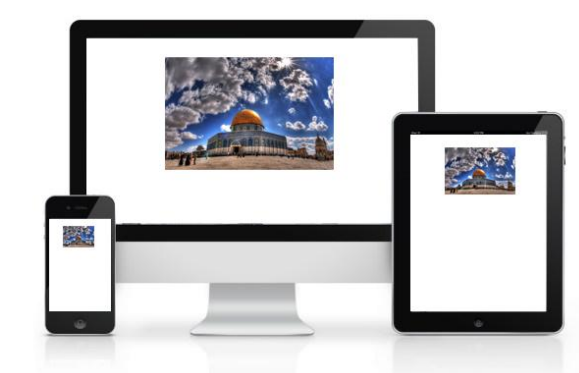
\includegraphics[keepaspectratio,width=\linewidth,height=\halfh]
        {relative.png}
        
        \caption[Relative Image Dimensions]{
            Relative Image Dimensions.
        \imgcredit{Taken from research paper.}
        }
        \label{fig:TUG}
        \end{figure}
%TODO SPECIFY LINK AL NE RADI MAMU MU
\newpage
\subsection{Cropping} 

Another option is cropping, which crops the picture to a certain width
with the help of CSS. 

\begin{figure}[h!]
    \centering
    \subfloat[%  the % chars remove implicit spacing
    Picture with original size
    ]
    {%
    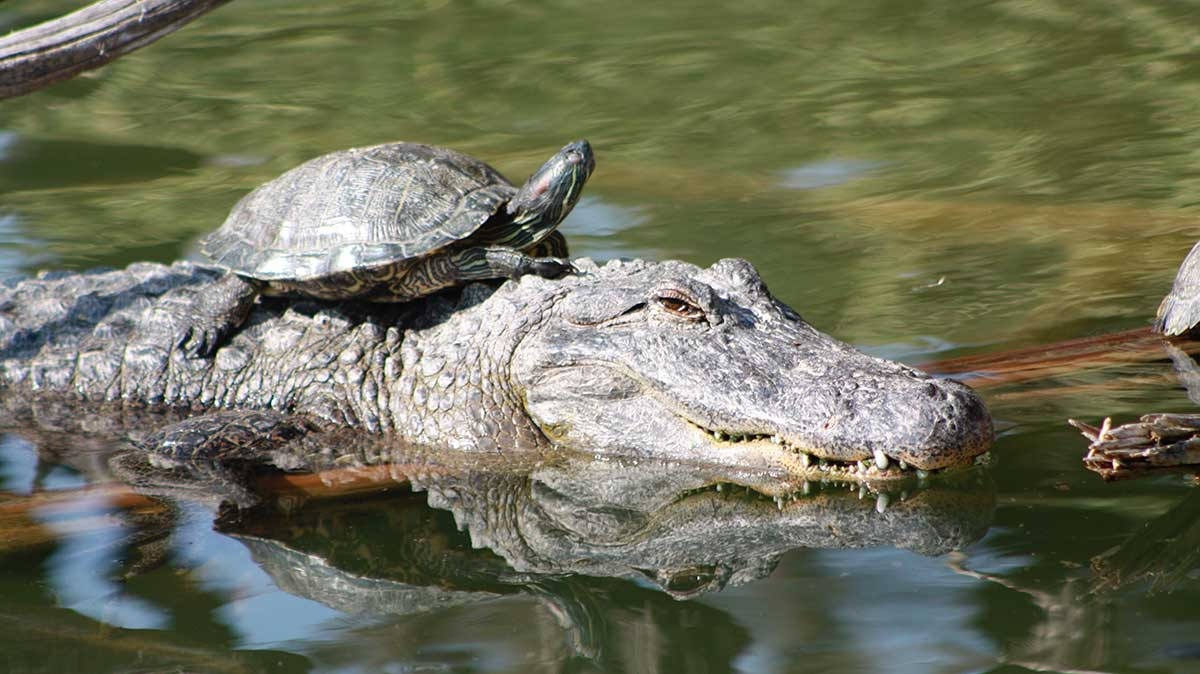
\includegraphics[width=\linewidth]
    {alig1.jpg}%
    \label{alig1}%
    }
    \hfill
    \subfloat[%
    Picture when cropped 
    ]
    {%
    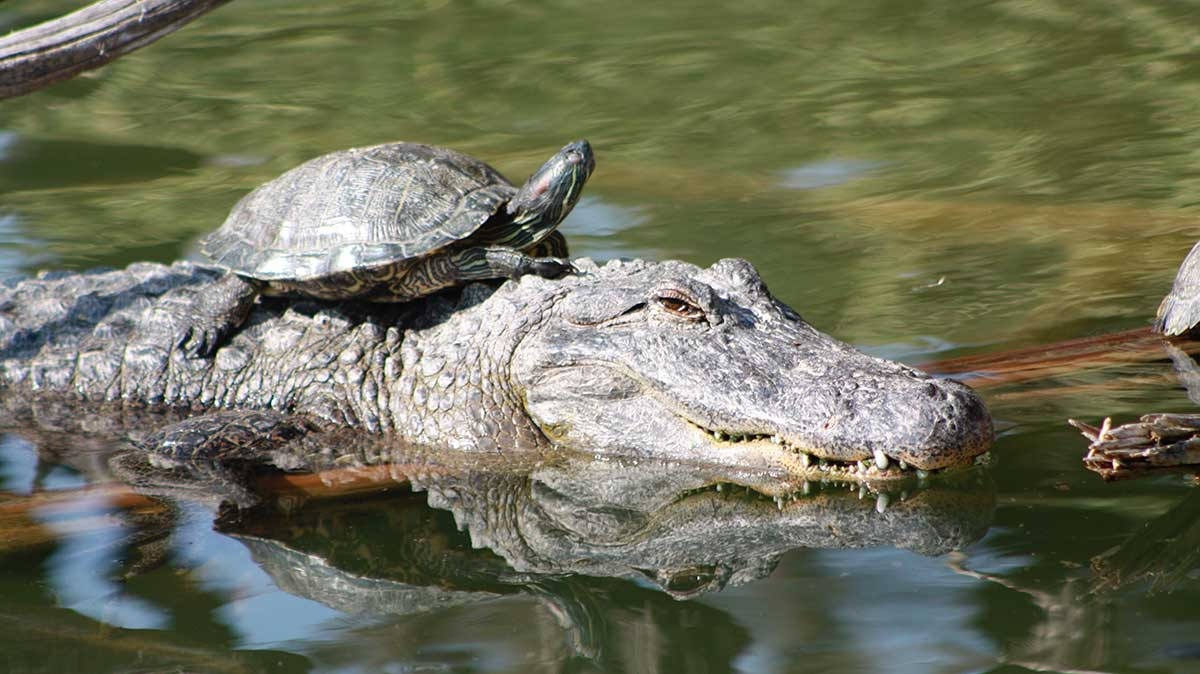
\includegraphics[width=0.45\linewidth]
    {alig2.jpg}%
    \label{alig2}%
    }
    
    \caption[Image Cropping]
    {
      Image cropping.
    \imgcredit{https://alligator.io/css/cropping-images-object-fit/.}
    }
    \label{figWhol}
\end{figure}

In this Figure above, it can be obviously seen that the result of tweaking the image a bit.
With just a few CSS commands, it is possible to crop the picture and if someone is browsing the
web site with a smaller device, the image does not have to be hidden, just its' size is changed.

\begin{lstlisting}[%
    language = HTML, 
    xleftmargin=0cm,              % no extra margins for floats
    xrightmargin=0cm,             % no extra margins for floats
    language=biblatex,
    basicstyle=\footnotesize\ttfamily,
    frame=shadowbox,
    numbers=left,
    label=list:BibACMIEEE,
     stringstyle=\color{blue}
    ,
]
    % An example of a media query, where one can say that for a screen of size 850px or less, the background is black:

    figure{
     width:300px; /*container-width*/
     overflow:hidden; /*hide bounds of image */
     margin:0;   /*reset margin of figure tag*/
   }
   figure img{
     display:block; /*remove inline-block spaces*/
     width:100%; /*make image streatch*/
}
\end{lstlisting}
Taken from
\imgcredit{https://medium.com/@elad/how-to-crop-images-with-css-b8471d402b16.}   

\cleardoublepage
%----------------------------------------------------------------
%
%  File    :  survey-browsers.tex
%
%  Author  :  Keith Andrews, IICM, TU Graz, Austria
%
%  Created :  27 May 1993
%
%  Changed :  16 Nov 2010
%
%----------------------------------------------------------------


\chapter{HTML Tables}

\label{HTML5 Tables}

In case of having much data to display, or data which is better of in a grid, HTML tables
are the best solution available. Before, tables have been used mostly for the layout of
HTML web-sites and it is not a good practice to do so, mainly because of two things:


$\bullet$ Semantically it is wrong

$\bullet$ Tables aren't as adaptable and flexible as divs'

\section{Structure of tables}

The basic structure of an HTML table starts with the \textit{<table>} tag. It is the starting
point for constructing a table. Now, HTML tables consist of columns and rows, like normal
tables. For rows, the tag  \textit{<tr>} is used, whereas for table header \textit{<th>} tag
is used. Normally, table headers are positioned in the center and are bold. For table cells
\textit{<td>} tag is used \parencite{7}.
\newpage

\begin{lstlisting}[%
    language = CSS,
    xleftmargin=0cm,              % no extra margins for floats
    xrightmargin=0cm,             % no extra margins for floats
    language=biblatex,
    basicstyle=\footnotesize\ttfamily,
    frame=shadowbox,
    numbers=left,
    label=list:BibACMIEEE,
    ,
]
    % An example of an HTML Table which demonstrates information about cars:
    <!DOCTYPE html>
<html>
<head>
	<title>Best Cars 2019</title>
</head>
<body>
<table class="table table-bordered table-hover table-condensed">
	<thead>
		<tr>
			<th title="Field #1">Car</th>
			<th title="Field #2">Manufacturer</th>
			<th title="Field #3">Engine Size</th>
			<th title="Field #4">Cylinders</th>
			<th title="Field #5">Horsepower</th>
			<th title="Field #6">Torque</th>
			<th title="Field #7">Compresion Ratio</th>
			<th title="Field #8">Miles per gallon</th>
			<th title="Field #9">Price</th>
		</tr>
	</thead>
	<tbody>
		<tr>
			<td>2019 Acura RDX</td>
			<td>Acura</td>
			<td>2.00L</td>
			<td align="right">4</td>
			<td align="right">272</td>
			<td align="right">280</td>
			<td>9.8:1</td>
			<td align="right">28</td>
			<td>€33,600.00</td>
		</tr>
		<tr>
			<td>2019 Ford Ranger</td>
			<td>Ford</td>
			<td>2.30L</td>
			<td align="right">4</td>
			<td align="right">270</td>
			<td align="right">310</td>
			<td>10.0:1</td>
			<td align="right">21</td>
			<td>€21,800.00</td>
		</tr>
	</tbody>
</table>

</body>
</html>

\end{lstlisting}

Now, there exist some other tags which can be used for HTML5 tables:

$\bullet$ <thead> - Table header, it is used to point out single or multiple rows
of a table, which do not contain table data but column labels \parencite{8}.

$\bullet$ <tbody> - Table body, it is used to point out <tr> elements. Position this tag
always after <thead>, but it can also come after or before <tfoot> \parencite{8}.

$\bullet$ <tfoot> - Table footer, it is used to point out single or multiple <tr> elements
where those elements are presenting an overview  of the data in the table \parencite{8}.

$\bullet$ <caption> - Table caption, as the name already says, can be used to specify table caption.
Can be put on the bottom of the CSS document.

$\bullet$ <col> - While using col and some other keyword, for example, align, it is possible direct
the alignment of text in the table. There are other keywords whom can be used to adjust colors, width
and many other things of table columns.





\section{Good Table Design}
Now, there are certain guidelines which can help a developer, or if that person can be called that way,
table maintainer, make a table and its design better. By that is meant that there are some interesting ways
where a little of simple CSS can be used to your advantage to make your table stand out.


\subsection{Alternate row highlighting}
When presented a table with a lot of entries, it can be hard to look at. Scrolling through numerous rows can be frustrating.
With this CSS trick, it can be a bit easier, atleast for the eyes if nothing else. The idea is to color every even row, while leaving
the odd ones in tact.
As said, it is pretty simple, and requires only two lines of CSS, but also pretty useful.


\begin{lstlisting}[%
    language = HTML,
    xleftmargin=0cm,              % no extra margins for floats
    xrightmargin=0cm,             % no extra margins for floats
    language=biblatex,
    basicstyle=\footnotesize\ttfamily,
    frame=shadowbox,
    numbers=left,
    label=list:BibACMIEEE,
     stringstyle=\color{blue}
    ,
]
    % An example of using simple CSS to color table rows:

	table.alt tr:nth-child(even) {background: #CCC}
	table.alt tr:nth-child(odd) {background: #FFF}

\end{lstlisting}


And now, at the end, this is the final result:
\begin{figure}[H]
    \centering

    {%
    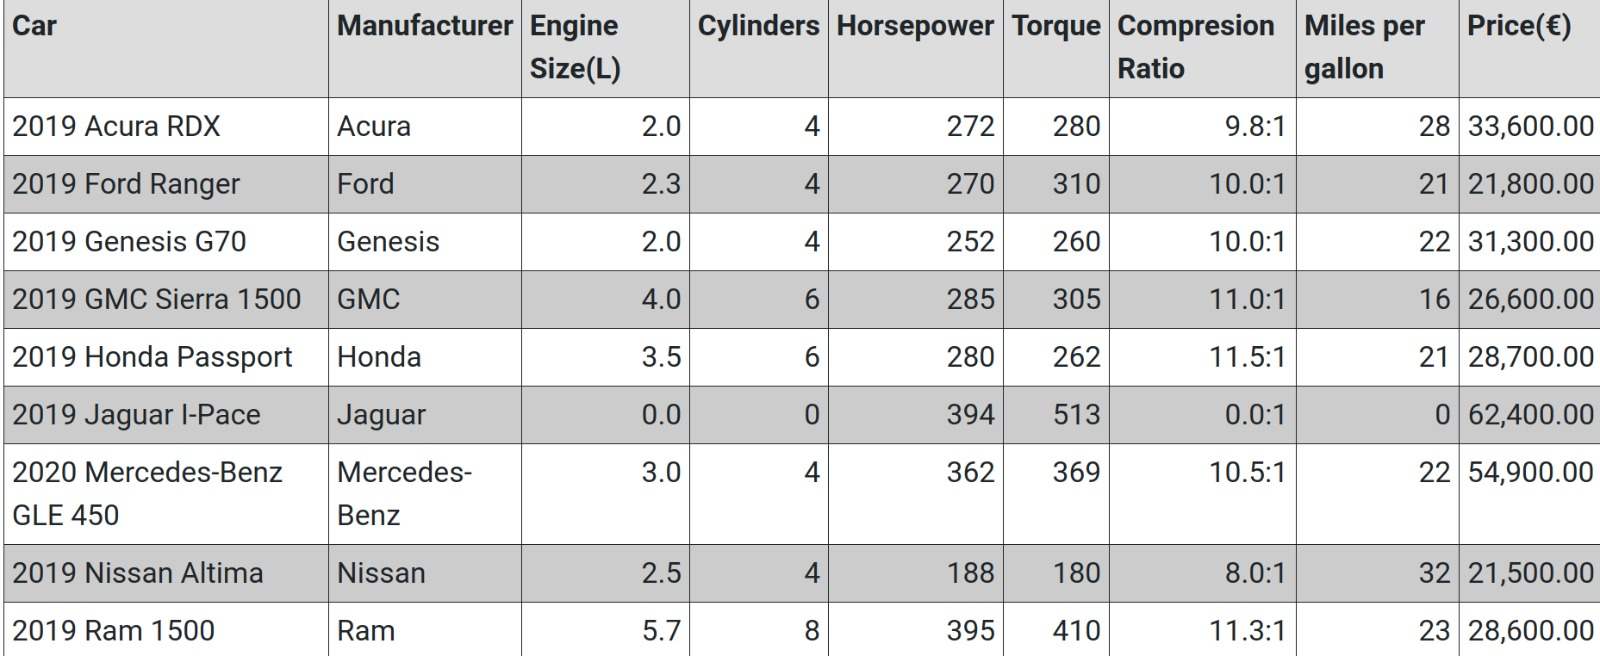
\includegraphics[width=\linewidth]
    {alt_t.jpeg}%
    \label{alig1}%
    }


    \caption[Alternate row highlighting]
    {

    \imgcredit{Screenshot taken by the author.}
    }
    \label{figWhol}
\end{figure}


\newpage
\subsection{Current Row Highlighting}
Now again, talking about a big table, and going through it, one may
easily becomes lost and wouldn't know in which row he is at the moment, which can be
pretty stressful. Again with the help of some CSS, the lives of the users' is made easier.

\begin{lstlisting}[%
    language = HTML,
    xleftmargin=0cm,              % no extra margins for floats
    xrightmargin=0cm,             % no extra margins for floats
    language=biblatex,
    basicstyle=\footnotesize\ttfamily,
    frame=shadowbox,
    numbers=left,
    label=list:BibACMIEEE,
     stringstyle=\color{blue}
    ,
]
    % An example of using simple CSS to highlight table rows:

	table {
      overflow: hidden;
	}

	tr:hover {
	  background-color: #ffa;
	}

	td, th {
	  position: relative;
	}
	td:hover::after,
	th:hover::after {
	  content: "";
	  position: absolute;
	  background-color: #ffa;
	  left: 0;
	  width: 100%;
	  z-index: -1;
	}

\end{lstlisting}


And again, it is shown how a small amount of CSS can be helpful.
The result:
\begin{figure}[H]
    \centering

    {%
    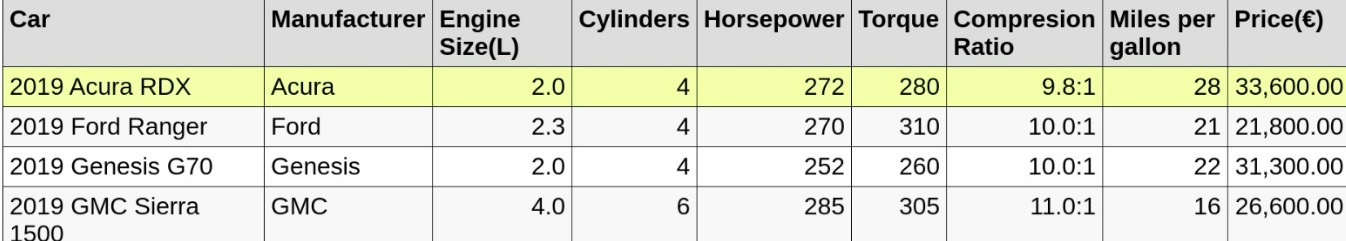
\includegraphics[width=\linewidth]
    {current_hl.jpeg}%
    \label{alig1}%
    }


    \caption[Current Row Highlighting]
    {

    \imgcredit{Screenshot taken by the author.}
    }
    \label{figWhol}
\end{figure}

\subsection{Expandable Areas}
Should we have any further information available about a table's object,
making the row clickable and showing the extra information then, is a better
alternative than trying to cram everything inside the table. In the following code sipped
we see how we put addtion data in html code.
\newpage
\begin{lstlisting}[%
    language = HTML,
    xleftmargin=0cm,              % no extra margins for floats
    xrightmargin=0cm,             % no extra margins for floats
    language=biblatex,
    basicstyle=\footnotesize\ttfamily,
    frame=shadowbox,
    numbers=left,
    label=list:BibACMIEEE,
     stringstyle=\color{blue}
    ,
]
<tr>
      <td>2019 Acura RDX</td>
      <td>Acura</td>
      <td style="text-align: right">2.0</td>
      <td style="text-align: right">4</td>
      <td style="text-align: right">272</td>
      <td style="text-align: right">280</td>
      <td style="text-align: right">9.8:1</td>
      <td style="text-align: right">28</td>
      <td style="text-align: right">33,600.00</td>
    </tr>
    <tr>
      <td colspan="5">
        <h4>Additional information about the car</h4>

        <ul>
          <li><a href="https://en.wikipedia.org/wiki/Acura_RDX">Acura RDX</a>
          </li>
          <li><a href="https://www.acura.ca/rdx">Acura RDX official webpage</a>
          </li>
        </ul>
      </td>
    </tr>
    <tr>
\end{lstlisting}
To implement this table feature we need to implement the combination of javascript and
css. In the further codes sipped the javascript and css code can be reviewed.
JavaScript Code
\begin{lstlisting}[%
    language = HTML,
    xleftmargin=0cm,              % no extra margins for floats
    xrightmargin=0cm,             % no extra margins for floats
    language=biblatex,
    basicstyle=\footnotesize\ttfamily,
    frame=shadowbox,
    numbers=left,
    label=list:BibACMIEEE,
     stringstyle=\color{blue}
    ,
]
<script type="text/javascript">
$(document).ready(function(){

  $("#report tr:odd").addClass("odd");
  $("#report tr:not(.odd)").hide();
  $("#report tr:first-child").show();

  $("#report tr.odd").click(function () {
    var trToToggle = $(this).next("tr");
    $("#report tr:not(.odd)").not(trToToggle).hide();
    $("#report tr:first-child").show();
    $(trToToggle).toggle();
    $(this).find(".arrow").toggleClass("up");
  });
})
</script>

\end{lstlisting}
\newpage

\begin{lstlisting}[%
    language = HTML,
    xleftmargin=0cm,              % no extra margins for floats
    xrightmargin=0cm,             % no extra margins for floats
    language=biblatex,
    basicstyle=\footnotesize\ttfamily,
    frame=shadowbox,
    numbers=left,
    label=list:BibACMIEEE,
     stringstyle=\color{blue}
    ,
]
#report {
    border-collapse:collapse;
}
#report h4 {
    margin:0px;
    padding:0px;
}
#report img {
    float:right;
}
#report ul {
    margin:10px 0 10px 40px;
    padding:0px;
}
#report th {
    background:#7CB8E2  repeat-x scroll center left;
    color:#fff;
    padding:7px 15px;
    text-align:left;
}
#report td {
    background:#C7DDEE none repeat-x scroll center left;
    color:#000;
    padding:7px 15px;
}
#report tr.odd td {
    cursor:pointer;
}
#report div.arrow {
    background:transparent url(arrows.png) no-repeat scroll 0px -16px;
    width:16px;
    height:16px;
    display:block;
}
#report div.up {
    background-position:0px 0px;
}
\end{lstlisting}

Now we will see how it look like in partice on html page. It is compiled localy. In the figure 2.3
we can see how our table look when we see it in html page.
\begin{figure}[H]
    \centering

    {%
    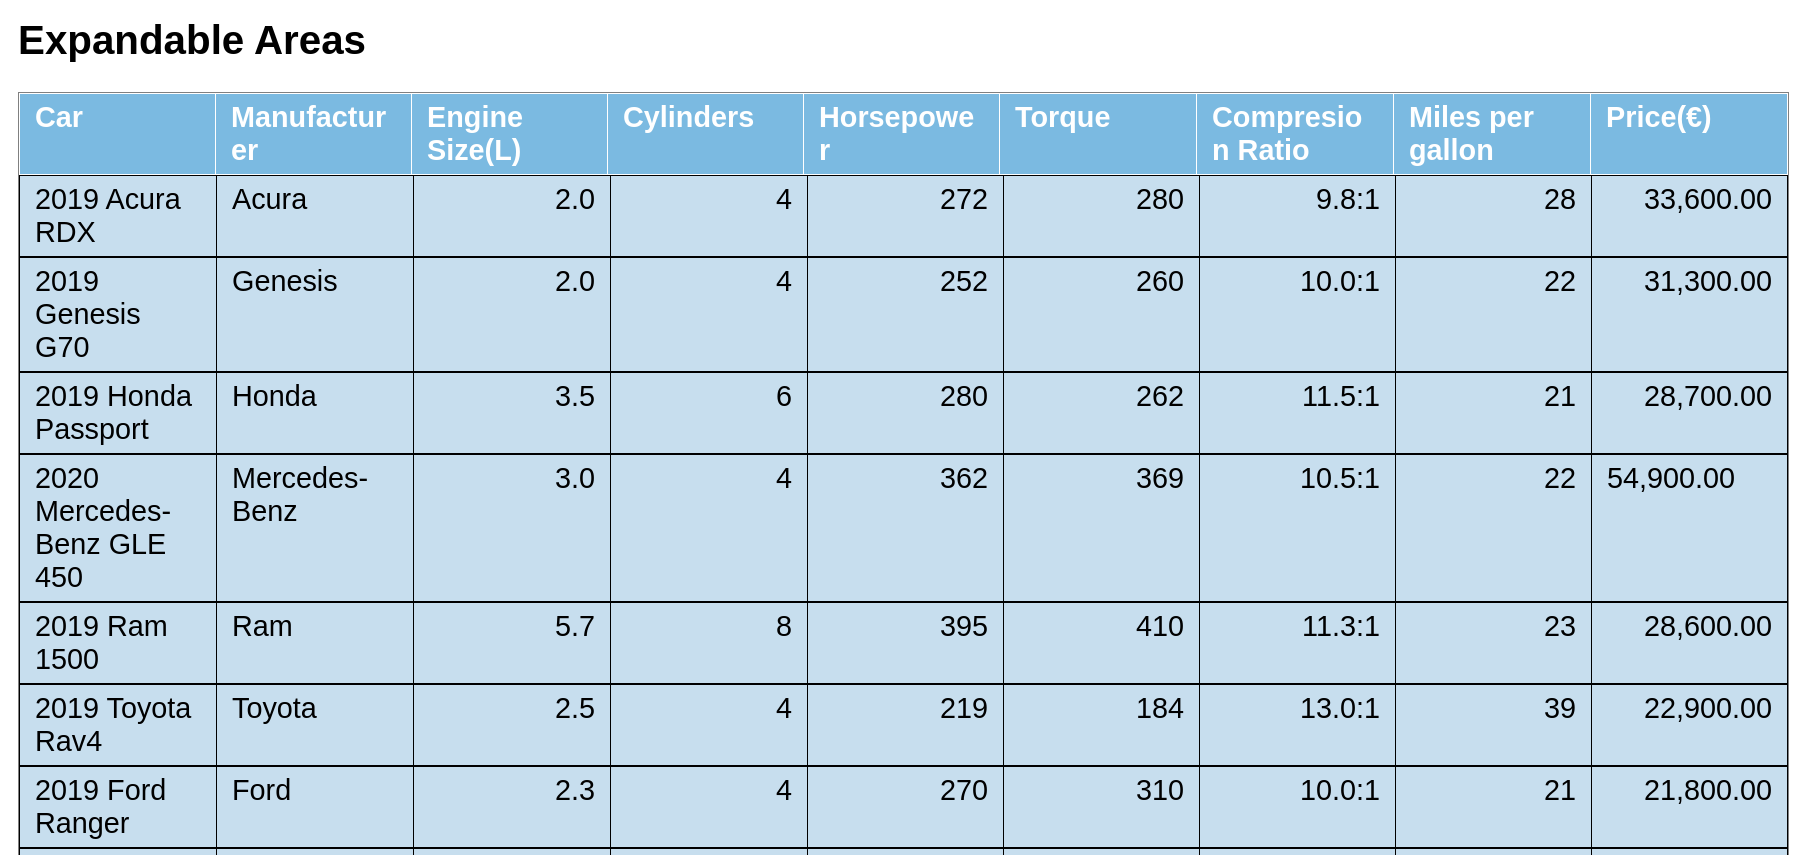
\includegraphics[width=\linewidth]
    {expandable_area_before.png}%
    \label{alig1}%
    }


    \caption[Expandable Areas]
    {

    \imgcredit{Screenshot taken by the author.}
    }
    \label{figWhol}
\end{figure}
Pressing to some of cell in row or colums we get the additional infomrmation, that we defined
in html code. This is shown in the figure 2.4.
\begin{figure}[H]
    \centering

    {%
    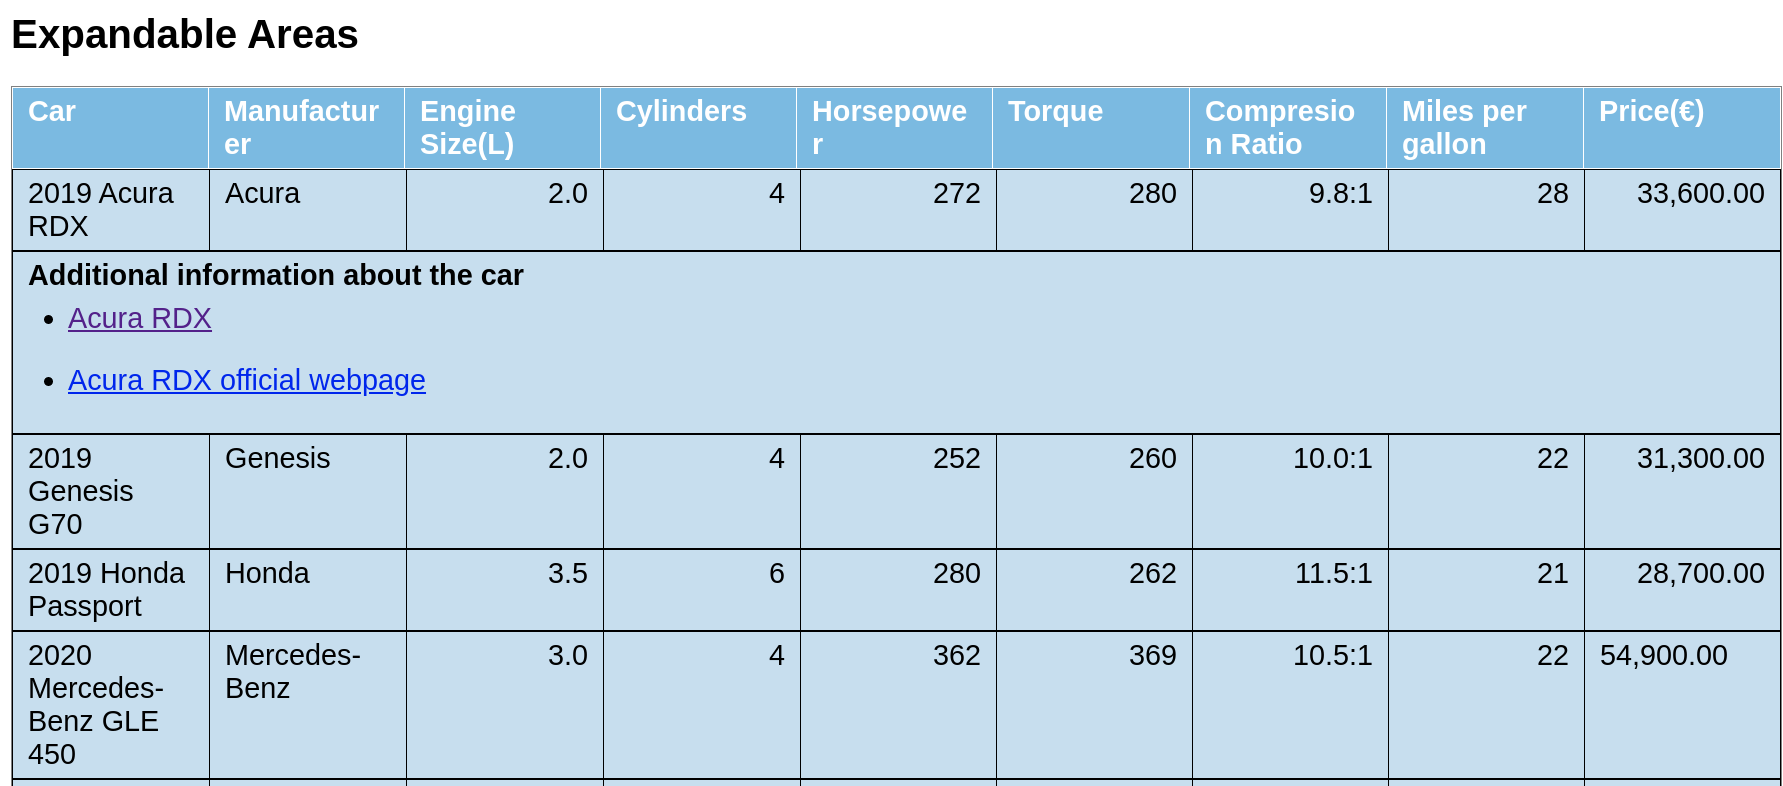
\includegraphics[width=\linewidth]
    {expandable_areas_after.png}%
    \label{alig1}%
    }


    \caption[Expandable Areas]
    {

    \imgcredit{Screenshot taken by the author.}
    }
    \label{figWhol}
\end{figure}

\subsection{Pagination (With Sort and Search)}
The amount of data increases every second, over 2.5 quintillion bytes of data are made every day and there is also estimation
 that in 2020 will be created 1.7MB of data in every second for each person in the world\parencite{PG_2}.
\newline
Tables are sometimes one of the possible places for saving large sets of data.
This type of tables should consists of different types of features that enables users easier operations of maintaining.
\newline
Were the table be too long, it can be divided into 'pages', and then certain amount of rows is viewed at a time.
\newline

An example of good table design with different features is called pagination, because the most important feature of this technique is pagination.
With this feature is possible to determine the number of rows per page, previous  and next page navigation are also available.
Every user has also possibility to filter results by text search and in this way find the desired row.
There is also possibility to sort table content in an descending or ascending order.

This solution works for following browsers:
\newline $\bullet$ Google Chrome
\newline $\bullet$ Mozzila Firefox
\newline $\bullet$ Internet Explorer
\newline $\bullet$ Opera
\newline $\bullet$ Microsoft Edge

For the implementation plug-in for the jQuery Javascript library called DataTables is used\parencite{PG_1}.


\begin{lstlisting}[%
    language = HTML,
    xleftmargin=0cm,              % no extra margins for floats
    xrightmargin=0cm,             % no extra margins for floats
    language=biblatex,
    basicstyle=\footnotesize\ttfamily,
    frame=shadowbox,
    numbers=left,
    label=list:BibACMIEEE,
     stringstyle=\color{blue}
    ,
]
    % An example of using Javascript plugin DataTable():
    %Include these two files in order to include additional advanced features to any HTML table
    %cdn.datatables.net/1.10.20/css/jquery.dataTables.min.css
    %cdn.datatables.net/1.10.20/js/jquery.dataTables.min.js

    $(document).ready(function(){
        $('#myTable').dataTable(); //this plugin provides searching, sorting and pagination
 });

\end{lstlisting}

Table is initilaized with "myTable" id and this id is used in
 ready function() to assign dataTable funcionality to our HTML table instance\parencite{PG}.

Following image represents html table with sorted Price column and 10/12 entries:
\begin{figure}[H]
    \centering

    {%
    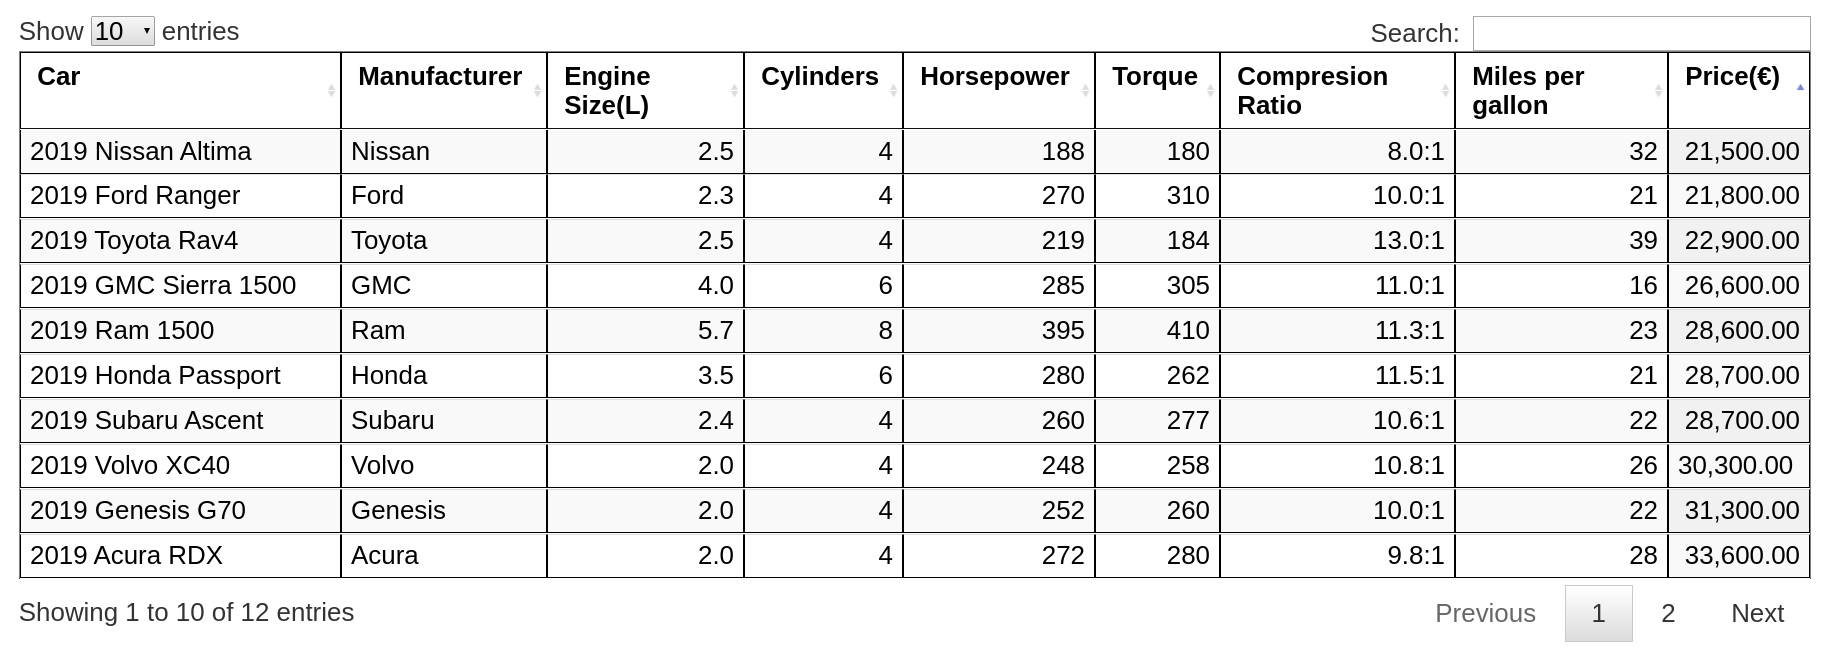
\includegraphics[width=\linewidth]
    {pagination_2.png}%
    \label{alig1}%
    }


    \caption[Pagination with sort option]
    {

    \imgcredit{Screenshot taken by the author.}
    }
    \label{figWhol}
\end{figure}

Following image represents html table with searched term:
\begin{figure}[H]
    \centering

    {%
    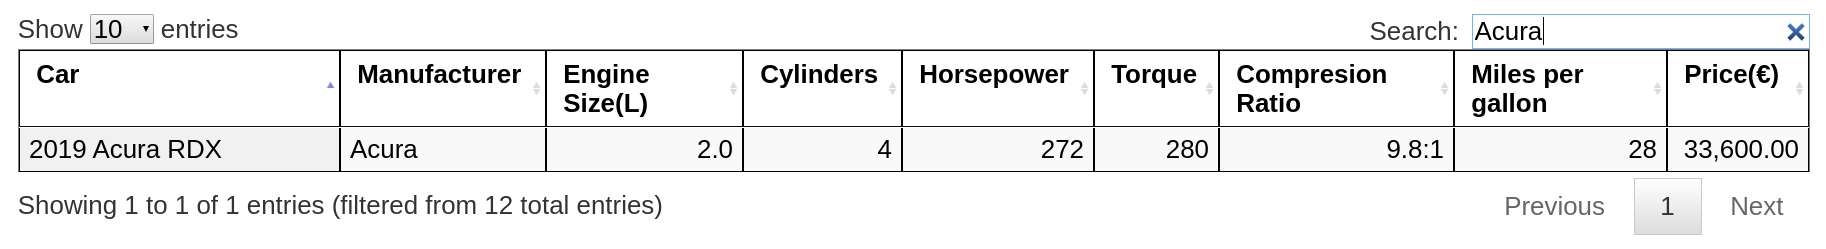
\includegraphics[width=\linewidth]
    {pagination_1.png}%
    \label{alig1}%
    }


    \caption[Pagination with search option]
    {

    \imgcredit{Screenshot taken by the author.}
    }
    \label{figWhol}
\end{figure}

\newpage

\section{Responsive Tables}

Due to the increasing amount of screens and their varying shapes, sizes,
and developers' space allocation when designing and implementing tables,
responsive table techniques have been 'developed' by manipulating the table's
columns and rows to provide an optimal experience for users across most mediums. It means the row and
columns can be repositioned,
resized, collapsed, minimized, etc..
Here are some techniques we would like to decsribe in the following chapter:
\newline
\newline $\bullet$ Hidden Columns - Selected by User
\newline $\bullet$ Horizontal Scroll
\newline $\bullet$ Fixed Header
\newline $\bullet$ Flip Scroll
\newline $\bullet$ User Resizeable Columns
\newline $\bullet$ Long Two Column

In literatury the mostly is find online("on internet") there are a lot of techniques i.e.
there are a lot of names for very similar or the same techniques. We tried to take the best ones,
to name it on most resonable way and to describe them.

\newpage
\section{Responsive Tables Techniques}



Data tables can contain many information, which makes displaying that data quite messy and hard to
look at. So by using responsive design, a big favor is done to the clients,
by adjusting the table according to their devices. One idea would be to minimize the table, but if the user is looking
at the table from his mobile device, he would have to zoom in, which is not that useful to him, because then again he would need to scroll
to view the whole table \parencite{9}.

\begin{figure}[H]
    \centering

    {%
    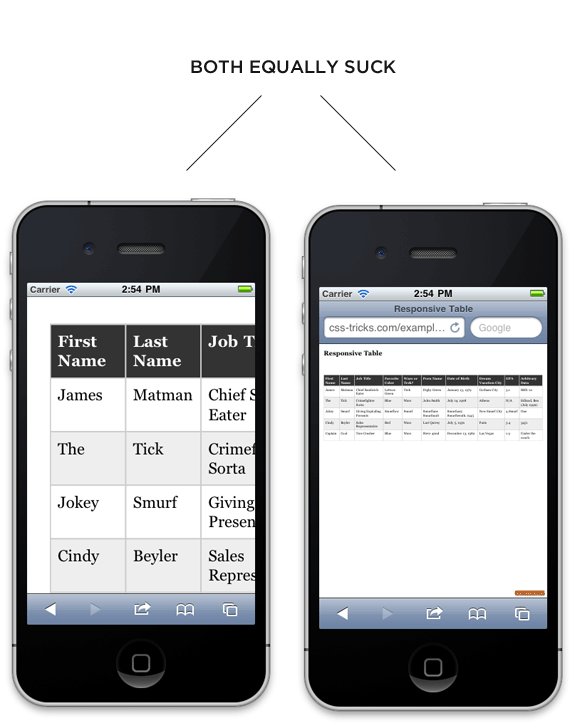
\includegraphics[width=\linewidth]
    {zoom_1.png}%
    \label{alig1}%
    }


    \caption[Before reponsive]
    {

    \imgcredit{https://css-tricks.com/responsive-data-tables/.}
    }
    \label{figWhol}
\end{figure}

As seen in the figure above, both options do not really look nor do as any good.
So, by using some simple CSS it is possible to fix that problem. With the help of the mentioned
media queries, it is possible to specify for which device sizes, which settings should be used.

\begin{lstlisting}[%
    language = HTML,
    xleftmargin=0cm,              % no extra margins for floats
    xrightmargin=0cm,             % no extra margins for floats
    language=biblatex,
    basicstyle=\footnotesize\ttfamily,
    frame=shadowbox,
    numbers=left,
    label=list:BibACMIEEE,
     stringstyle=\color{blue}
    ,
]
    % An example of using simple CSS with media queries on how to achieve Responsive Design:

    @media
only screen and (max-width: 760px),
(min-device-width: 768px) and (max-device-width: 1024px)  {

	/* Force table to not be like tables anymore */
	table, thead, tbody, th, td, tr {
		display: block;
	}

	/* Hide table headers (but not display: none;, for accessibility) */
	thead tr {
		position: absolute;
		top: -624.9375rem;
		left: -624.9375rem;
	}

	tr { border: 1px solid #ccc; }

	td {
		/* Behave  like a "row" */
		border: none;
		border-bottom: 1px solid #eee;
		position: relative;
		padding-left: 50%;
	}

	td:before {
		/* Now like a table header */
		position: absolute;
		/* Top/left values mimic padding */
		top: 0;
		left: 0.375rem;
		width: 45%;
		padding-right: 0.625rem;
		white-space: nowrap;
	}

\end{lstlisting}

\newpage
And now, the end result would be the following one:
\begin{figure}[H]
    \centering

    {%
    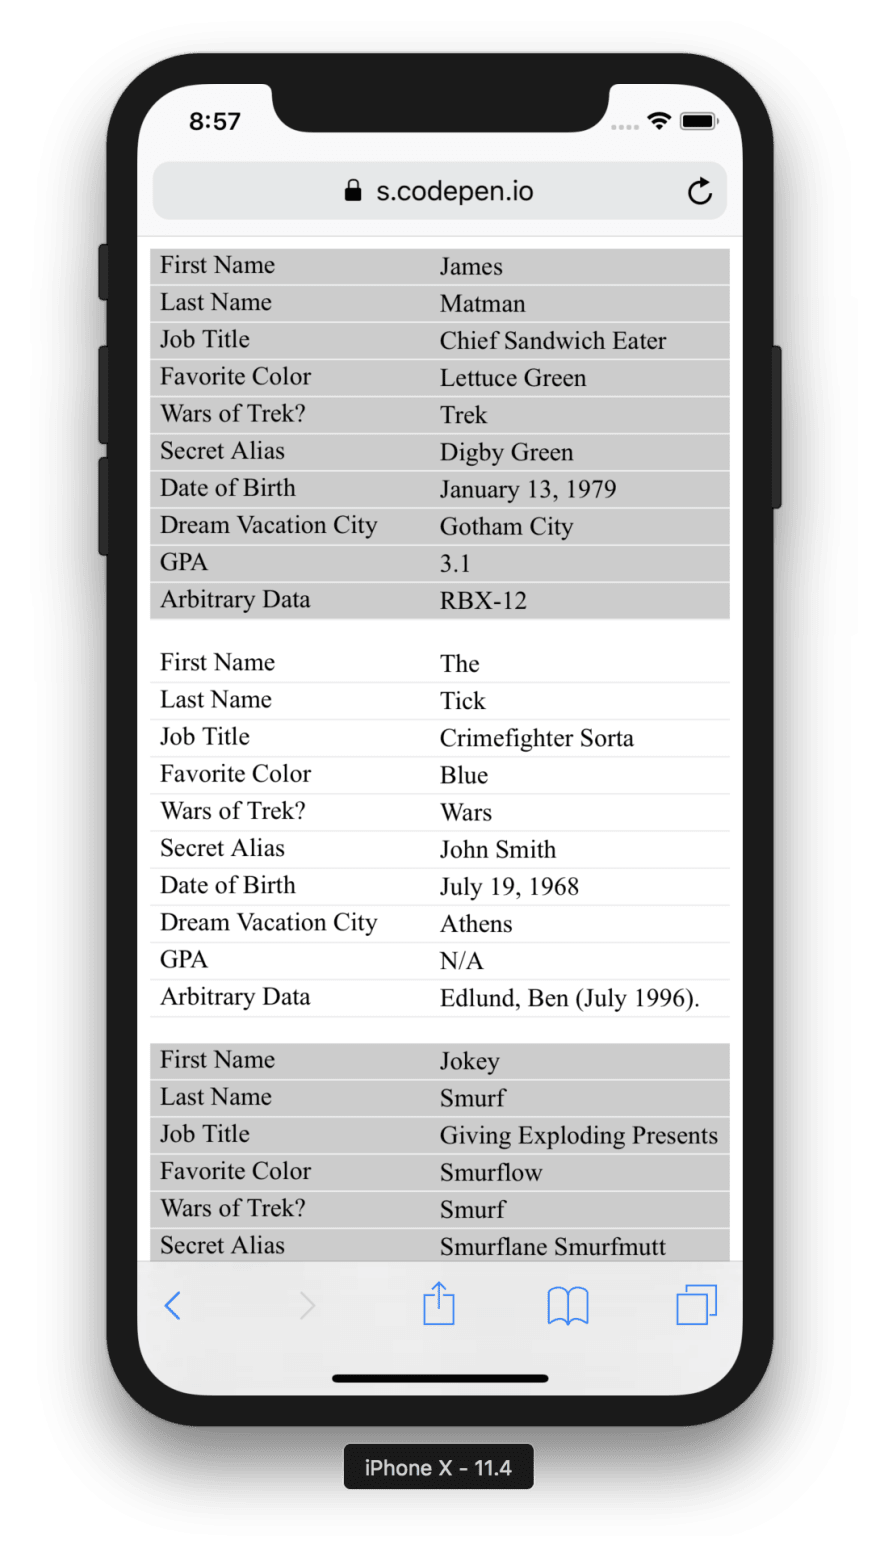
\includegraphics[width=0.45\linewidth]
    {zoom_3.png}%
    \label{alig1}%
    }


    \caption[After reposnsive]
    {

    \imgcredit{https://css-tricks.com/responsive-data-tables/.}
    }
    \label{figWhol}
\end{figure}

\newpage
\section{Horizontal Scroll}
When the allocated space is too small - horizontally, instead of hiding it, horizontal scroll bar just for the table is created and let the user scroll away.
\newline

Horizontal Scrolling represents a technique that resizes the table
into columns at small screen resoultion \parencite{HS_1}. The rows can be scrolled from left to right with fixed first row.
This is different from viewport scrolling as we scroll only through the table.
\newline

It is very useful technique when presenting large data
 sets with identifiers in the first column. Then is very easy for every user to compare data content with multiple identifiers\parencite{HS}.


This solution works for following browsers:
\newline $\bullet$ Google Chrome
\newline $\bullet$ Mozzila Firefox
\newline $\bullet$ Internet Explorer
\newline $\bullet$ Opera
\newline $\bullet$ Microsoft Edge
\newline
\newline It is impossible to find one size that fits all solution. Data comparing is very difficult on the small screens.
There are a lot of possible workarounds for this issue, but no one can solve this problem \parencite{HS_1}.
Our implementation of horizontal scrolling creates table elements scrollable, but also can not solve the issue to the end\parencite{HS_1}.
All important css-properties that creates a responsive table with horizontal scrolling are explained.

\begin{lstlisting}[%
    language = HTML,
    xleftmargin=0cm,              % no extra margins for floats
    xrightmargin=0cm,             % no extra margins for floats
    language=biblatex,
    basicstyle=\footnotesize\ttfamily,
    frame=shadowbox,
    numbers=left,
    label=list:BibACMIEEE,
     stringstyle=\color{blue}
    ,
]
.rtable {

    display: inline-block;
    vertical-align: top;
    max-width: 100%;

    overflow-x: auto;

    // optional - looks better for small cell values
    white-space: nowrap;

    border-collapse: collapse;
    border-spacing: 0;
}

\end{lstlisting}

This css code represents css class .rtable used in the case when container is not resized.
With display: inline-block all items are listed horizontally instead of vertically.
Vertical-align property maintains how elements set next to each other in a line.
The overflow property determines whether to crop content or to add scroll bars (along the x-axis) when a table's content is too big to satisfy some screen resolution.
We can use white-space: nowrap property as optional for small cell values.
Css border properties are used to control borders into a table\parencite{HS_1}.

Following image represents html table with horizontal scroll:

\begin{figure}[H]
    \centering

    {%
    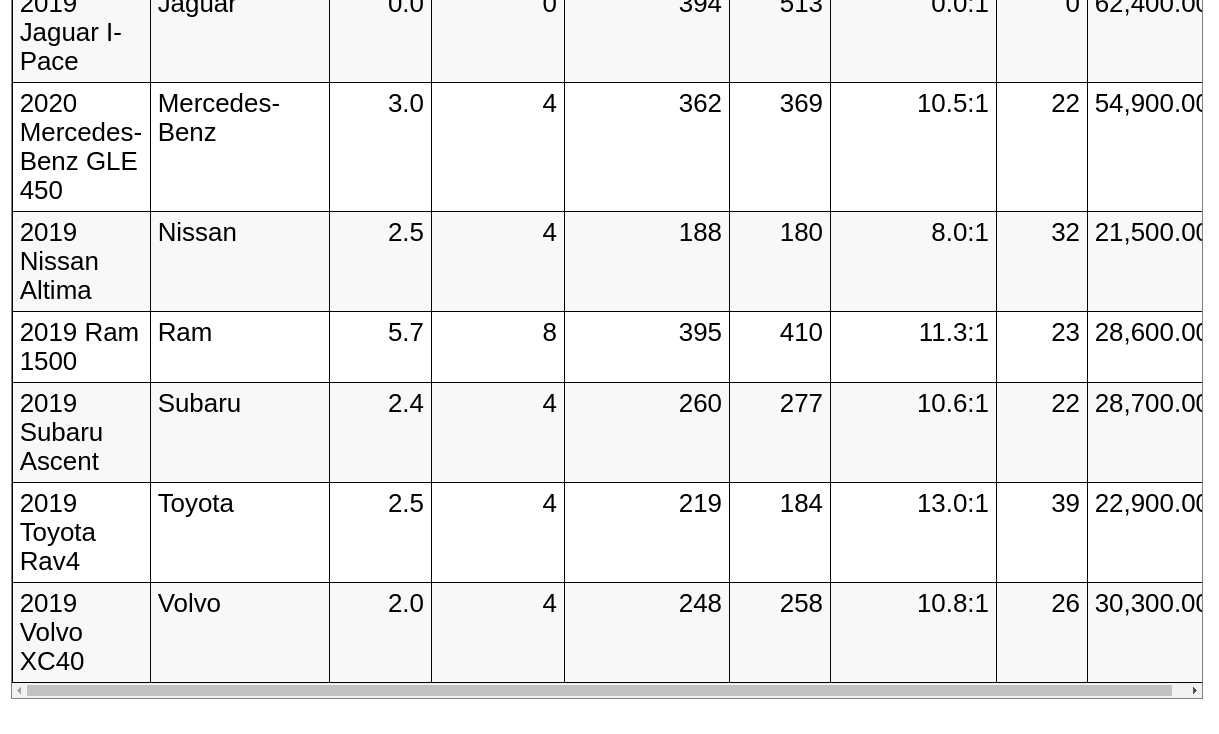
\includegraphics[width=1\linewidth]
    {horizontal.png}%
    \label{alig1}%
    }


    \caption[Horizontal Scroll]
    {

    \imgcredit{Screenshot taken by the author.}
    }
    \label{figWhol}
\end{figure}

\newpage
\section{Fixed Header}
When the table is vertically long, the table's header is fixed to the top of the table's view.
As we scroll down, the table's header is kept always visible.
\newline

It is very useful to have the fixed header (first row fixed) on the top of the table, when presenting tables with a particularly larage data set.
This helps users to quickly determine what every column identify rather than need to scroll back to the top of the table every time.
\newline Fixed Header provides background on what column the user is on.
This is very effective feature that makes our life easier \parencite{HS}.

This solution works for following browsers:
\newline $\bullet$ Google Chrome
\newline $\bullet$ Mozzila Firefox
\newline $\bullet$ Internet Explorer
\newline $\bullet$ Opera
\newline $\bullet$ Microsoft Edge

\begin{lstlisting}[%
    language = HTML,
    xleftmargin=0cm,              % no extra margins for floats
    xrightmargin=0cm,             % no extra margins for floats
    language=biblatex,
    basicstyle=\footnotesize\ttfamily,
    frame=shadowbox,
    numbers=left,
    label=list:BibACMIEEE,
     stringstyle=\color{blue}
    ,
]
.fixedHeader tbody {
    display: block;
    overflow: auto;
    width: 100%;
}

.fixedHeader thead tr {
    display: table;
    width: 100%;
    table-layout: fixed;
}

.fixedHeader thead, .fixedHeader tbody tr {
    display: table;
    width: 100%;
    table-layout: fixed;
}

.fixedHeader thead {
    width: calc( 100% - 0.6em )
}

.fixedHeader td {
    width: 100%;
}

\end{lstlisting}

Tbody element is determined with the type of rendering box.
With overflow: auto scrollbar will appear along y-axis.
All thead and tbody rows will behave as table elements.
Fixed table layout algorithm is used to control table and column widths.
Width for almost every table element is static, just the header has non-static width \parencite{FH_1}.
The width of header is determined with calc() function and in this way is solved the main issue in this responsive technique\parencite{FH}.

Following image represents html table with fixed header:

\begin{figure}[H]
    \centering

    {%
    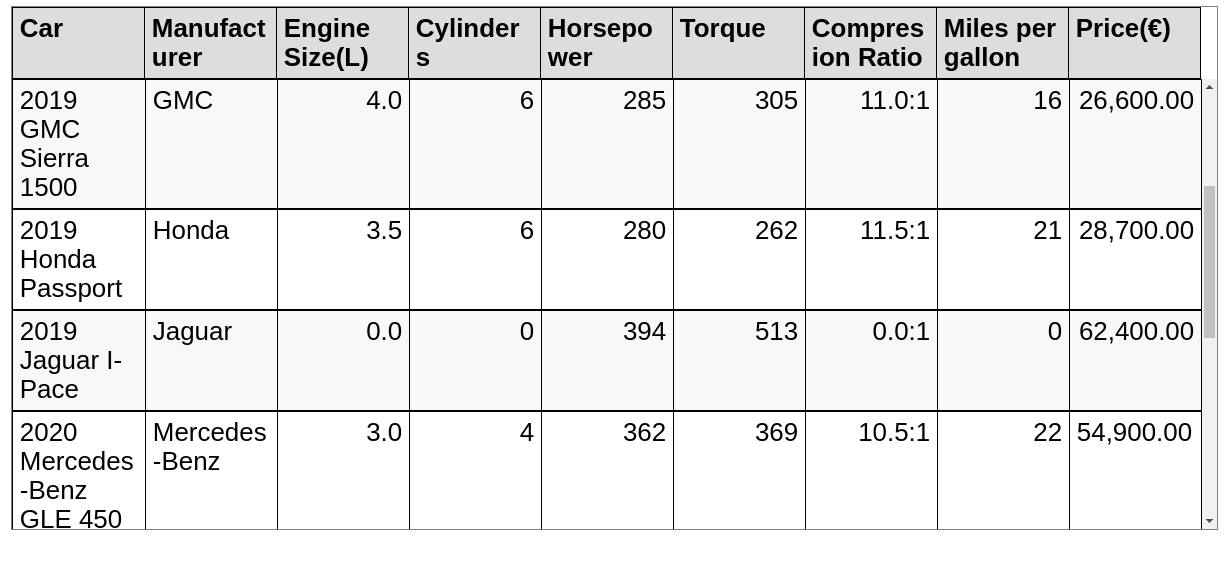
\includegraphics[width=1\linewidth]
    {fixed_header.png}%
    \label{alig1}%
    }


    \caption[Fixed Header]
    {

    \imgcredit{Screenshot taken by the author.}
    }
    \label{figWhol}
\end{figure}




\cleardoublepage
%----------------------------------------------------------------
%
%  File    :  survey-recc.tex
%
%  Author  :  Mirza Kabiljagic, Stefan Rajinovic, Aleksandar Stojicic,
%             Inti Gabriel Mendoza Estrada
%
%  Created :  27 May 20xx
%
%  Changed :  4 Dez 2019
%
%----------------------------------------------------------------


\chapter{Recommendation}
\label{chap:Recommendation}
 


\section{Recommendation}

Responsive tables must be able to efficiently and effectively display data. It is only through a combination of good table design and responsive techniques one is able to achieve this. 

For good table design, it is imperative that you include Alternate Row Highlighting. This is a very simple technique that works on every browser and is not only helpful to the user but to the developer as it adds positively to the aesthetics. 

For a ``Jack of all trades'' approach, we suggest the following responsive techniques: Long Two Column, and Fixed Header. You are able to apply this for the 3 main screen sizes: PC, tablet, and phone. Being able to apply Long Two Column to phone-sized screens (or tablets in vertical mode) and leave Fixed Header on the remaining two sizes (PC and tablets in horizontal mode) automatically eliminates one of the 3 sizes you have to take care of. 

Another thing to keep in mind is to attach the vertical scrollable feature of Fixed Header to the Long Two Column. This ensures that the space the table is taking up is exactly the one allocated to it. It goes without saying that if the table is too wide (horizontally), it should be horizontally scrollable.

The figure below shows these techniques working together.

\begin{figure}[tp]
    \centering
  
    {%
    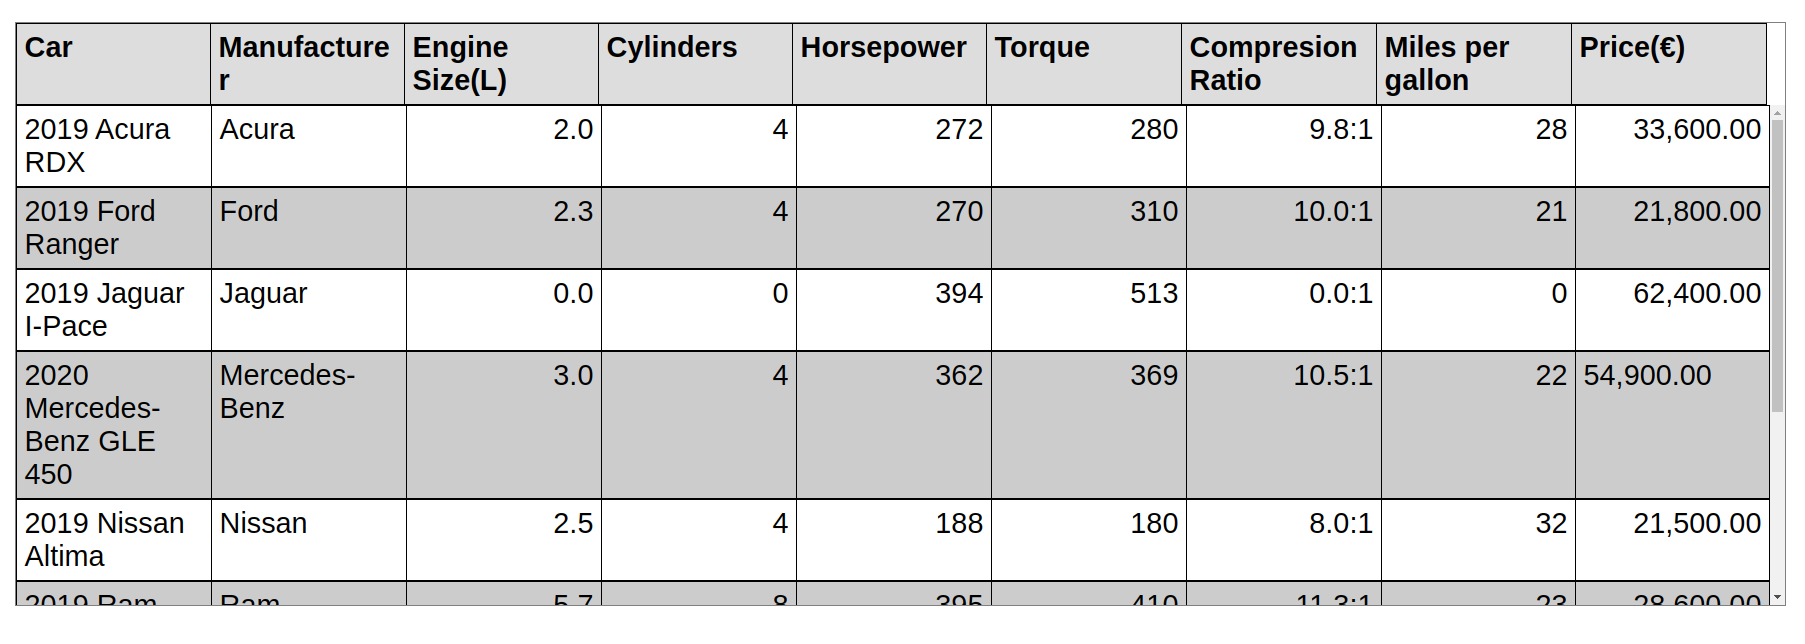
\includegraphics[width=1\linewidth]
    {images/recommendation_1.png}%
    \label{Recommendation 1}%
    }

    
    \caption[Recommendation Techniques 1]
    {
      
    \imgcredit{Screenshot taken by the author.}
    }
    \label{figRecc1}
\end{figure}

As you scroll through the table, notice the Fixed Header Technique in the image below.

\begin{figure}[tp]
    \centering
  
    {%
    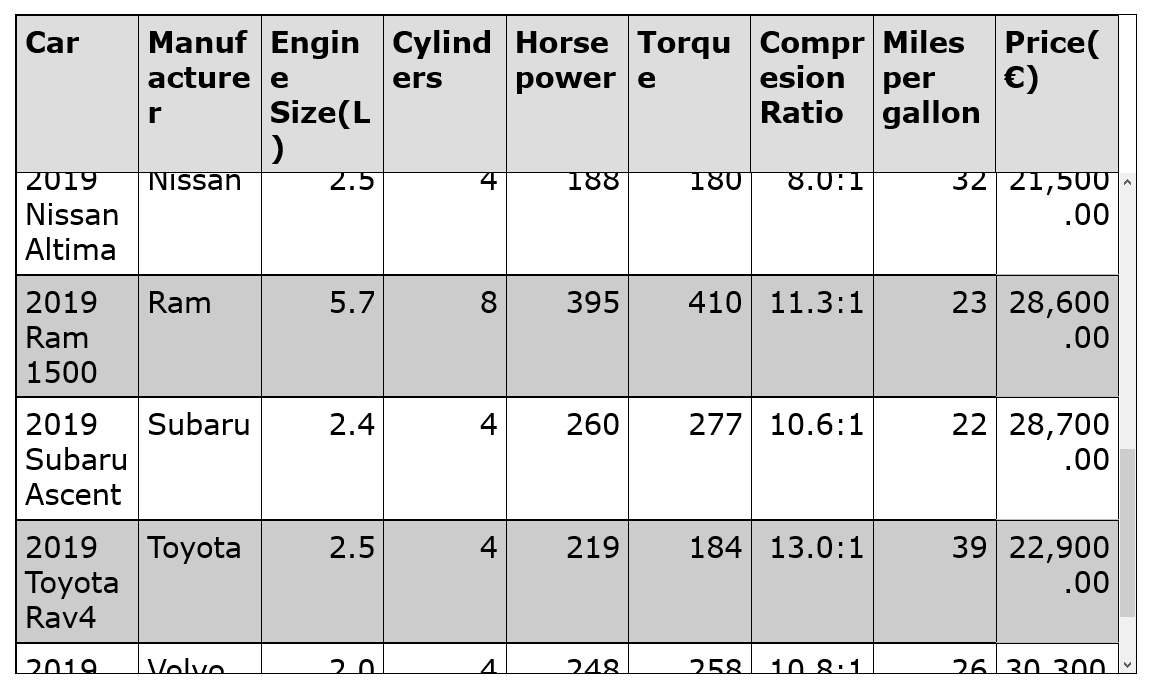
\includegraphics[width=1\linewidth]
    {images/recommendation_2.png}%
    \label{Recommendation 2}%
    }

    
    \caption[Recommendation Techniques 2]
    {
      
    \imgcredit{Screenshot taken by the author.}
    }
    \label{figRecc2}
\end{figure}

For small-sized screens, the technique that would ``kick in'' is shown in the image below. Notice the `creeping' second `minitable' in the bottom part.

\begin{figure}[tp]
    \centering
  
    {%
    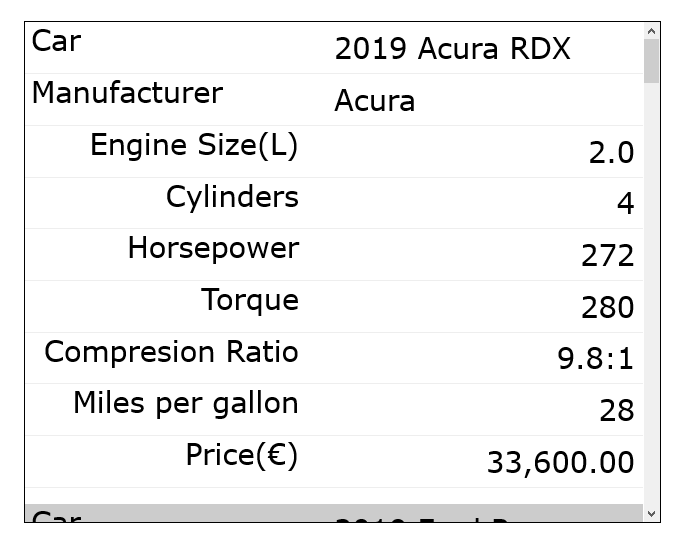
\includegraphics[width=1\linewidth]
    {images/recommendation_3.png}%
    \label{Recommendation 3}%
    }

    
    \caption[Recommendation Techniques 3]
    {
      
    \imgcredit{Screenshot taken by the author.}
    }
    \label{figRecc3}
\end{figure}





%\cleardoublepage
%%----------------------------------------------------------------
%
%  File    :  survey-style.tex
%
%  Author  :  Keith Andrews, ISDS, TU Graz, Austria
% 
%  Created :  27 May 1993
% 
%  Changed :  05 Nov 2018
% 
%----------------------------------------------------------------


\chapter{Language and Writing Style}

\label{chap:Style}


A comprehensive guide to writing British English is the New Oxford
Style Manual \parencite{NewOxfordStyleManual-3Ed}. The Economist Style
Guide \parencite{EconomistStyleGuide-12Ed} provides a compact indexed guide
to British English usage. \textcite{Zinsser-OnWritingWell-7Ed} is an
easy to read companion.

A comprehensive guide to writing American English is the Chicago
Manual of Style \parencite{ChicagoManualStyle-17Ed}.  The classic
compact reference for American English writing style and grammar is
\textcite{StrunkWhite-4Ed}. The original text is now available for
free online \parencite{Strunk-1Ed}. Another good free guide is
\textcite{NASAGuide}.

\textcite{Alley-CraftScientificWriting-4Ed} is a classic guide to
scientific writing. Other good ones include
\textcite{Booth-CraftResearch-4Ed} and
\textcite{Booth-CommunicatingScience-2Ed}.
%
\textcite{Zobel-WritingCompSci} and \textcite{BugsInWriting} are guides
specifically aimed at computer science students.
\textcite{Phillips-HowGetPhD} gives practical advice for PhD
students.
%
In 2017, Google made its internal Documentation Style   Guide
public \parencite{GoogleStyleGuide}.


Sections~\ref{sec:Clear} and \ref{sec:Gender} of this chapter are
adapted from the ACM CHI'94 conference language and writing style
guidelines.




\section{Paragraphs}

Sentences should be grouped into paragraphs by topic. A new paragraph
introduces a (slight) variation in topic. Paragraphs should consist of
\emph{several} sentences. In general, short paragraphs of only one or
two sentences should be merged topically with neighbouring paragraphs.
%
In \LaTeX, paragraphs are separated by a blank line. Random newlines
({\smaller\verb|\newline|} or {\smaller\verb|\\|}) should \emph{never}
be strewn throughout your text.

% In LaTeX, use a single-line comment to merge two short, but
% topically connected, paragraphs into one paragraph.





\section{Some Basic Rules of English}

There are a few basic rules of English for academic writing, which are
broken regularly by my students, particularly if they are non-native
speakers of English. Here are some classic and often encountered
examples:

\begin{itemize}

\item \emph{Never} use I, we, or you.

Write in the passive voice (third person).

\begin{tabular}{lp{0.9\linewidth}}
\dthumb & You can do this in two ways.   \\
\uthumb & There are two ways this can be done.  \\
\end{tabular}



\item \emph{Never} use he or she, his or her.

Write in the passive voice (third person).

\begin{tabular}{lp{0.9\linewidth}}
\dthumb & The user speaks his thoughts out loud.   \\
\uthumb & The thoughts of the user are spoken out loud.  \\
\end{tabular}

See Section~\ref{sec:Gender} for many more examples.



\item Stick to a consistent dialect of English. Choose either
  British or American English and keep to it throughout the
  whole of your thesis.



\item Do \emph{not} use slang abbreviations such as ``it's'',
  ``doesn't'', or ``don't''.

Write the words out in full: ``it is'', ``does not'', and ``do not''.

\begin{tabular}{lp{0.9\linewidth}}
\dthumb & It's very simple to\ldots       \\
\uthumb & It is very simple to\ldots       \\
\end{tabular}



\item Do \emph{not} use abbreviations such as ``e.g.'' or
  ``i.e.''. 

Write the words out in full: ``for example'' and ``that is''.

\begin{tabular}{lp{0.9\linewidth}}
\dthumb & \ldots in a tree, e.g. the items\ldots        \\
\uthumb & \ldots in a tree, for example the items\ldots   \\
\end{tabular}



\item Do \emph{not} use slang such as ``a lot of''.

\begin{tabular}{lp{0.9\linewidth}}
\dthumb & There are a lot of features\ldots       \\
\uthumb & There are many features\ldots       \\
\end{tabular}



\item Do \emph{not} use slang such as ``OK'' or ``big''.

\begin{tabular}{lp{0.9\linewidth}}
\dthumb & \ldots are represented by big areas.    \\
\uthumb & \ldots are represented by large areas.  \\
\end{tabular}



\item Do \emph{not} use slang such as ``gets'' or ``got''.

Use ``becomes'' or ``obtains'', or use the passive voice (third
person).

\begin{tabular}{lp{0.9\linewidth}}
\dthumb & The radius gets increased\ldots       \\
\uthumb & The radius is increased\ldots         \\
\end{tabular}

\begin{tabular}{lp{0.9\linewidth}}
\dthumb & The user gets disoriented\ldots       \\
\uthumb & The user becomes disoriented\ldots    \\
\end{tabular}




\item \emph{Never} start a sentence with ``But''.

Use ``However,'' or ``Nevertheless,''. Or consider joining the
sentence to the previous sentence with a comma.

\begin{tabular}{lp{0.9\linewidth}}
\dthumb & But there are numerous possibilities\ldots       \\
\uthumb & However, there are numerous possibilities\ldots  \\
\end{tabular}



\item \emph{Never} start a sentence with ``Because''.

Use ``Since'', ``Owing to'', or ``Due to''. Or turn the two
halves of the sentence around.




\item \emph{Never} start a sentence with ``Also''. Also should
be placed in the middle of the sentence.

\begin{tabular}{lp{0.9\linewidth}}
\dthumb & Also the target users are considered. \\
\uthumb & The target users are also considered. \\
\end{tabular}



\item Do \emph{not} use ``that'' as a connecting word.

Use ``which''.

\begin{tabular}{lp{0.9\linewidth}}
\dthumb & \ldots a good solution that can be computed easily.  \\
\uthumb & \ldots a good solution which can be computed easily.  \\
\end{tabular}




\item Do \emph{not} write single-sentence paragraphs. 

Avoid writing two-sentence paragraphs. A paragraph should contain at
least three, if not more, sentences.


\end{itemize}



% rules on the use of a comma in lists
% http://en.wikipedia.org/wiki/Serial_comma






\section{English Usage}
\label{sec:EnglishUsage}

I see these mistakes time and time again. Please do not
let me read one of them in your work.



\begin{itemize}

\item ``allows to'' is not English.

\begin{tabular}{lp{0.9\linewidth}}
\dthumb & The prototype allows to arrange components\ldots \\
\uthumb & The prototype supports the arrangement of components\ldots \\[1ex]
\dthumb & The system allows to identify issues\ldots \\
\uthumb & Issues can be identified by the system\ldots \\
\end{tabular}

% they allow to achieve



\item ``enables to'' is not English.

\begin{tabular}{lp{0.9\linewidth}}
\dthumb & it enables to recognise meanings\ldots \\
\uthumb & it enables the recognition of meanings\ldots \\
\end{tabular}



\item ``per default'' is not English.

Use ``by default''.

\begin{tabular}{lp{0.9\linewidth}}
\dthumb & Per default, the cursor is red. \\
\uthumb & By default, the cursor is red. \\
\end{tabular}




\item ``As opposed to'' is not English.

Use ``In contrast to''.

\begin{tabular}{lp{0.9\linewidth}}
\dthumb & As opposed to C, Java is object-oriented. \\
\uthumb & In contrast to C, Java is object-oriented. \\
\end{tabular}







\item ``actual'' \neqsym ``current'' 

If you mean ``aktuell'' in German, you probably mean
``current'' in English.

\begin{tabular}{lp{0.9\linewidth}}
\dthumb & The actual selection is cancelled. \\
\uthumb & The current selection is cancelled. \\
\end{tabular}



\item ``sensible'' \neqsym ``sensitive'' 

If you mean ``sensibel'' in German, you probably mean
``sensitive'' in English.

\begin{tabular}{lp{0.9\linewidth}}
\dthumb & Store sensible data securely. \\
\uthumb & Store sensitive data securely. \\
\end{tabular}




\item ``according'' \neqsym ``corresponding'' 

\begin{tabular}{lp{0.9\linewidth}}
\dthumb & For each browser, an according package is created. \\
\uthumb & For each browser, a corresponding package is created. \\
\end{tabular}




\item ``adopt'' \neqsym ``adapt'' 

To ``adopt something'' means ``etwas übernehmen'' in German.
To ``adapt something'' means ``etwas anpassen'' in German.

\begin{tabular}{lp{0.9\linewidth}}
\dthumb & This convention was adapted to show\ldots \\
\uthumb & This convention was adopted to show\ldots \\[1ex]
\dthumb & The diagram was adopted by the author. \\
\uthumb & The diagram was adapted by the author. \\
\end{tabular}




% countable and uncountable nouns
% https://english.stackexchange.com/questions/9439/amount-vs-number-vs-quantity
% https://dictionary.cambridge.org/grammar/british-grammar/amount-of-number-of-or-quantity-of

\item ``amount'' versus ``number'' 

Use ``number'' for countable things.
Use ``amount'' for uncountable things.

\begin{tabular}{lp{0.9\linewidth}}
\dthumb & The amount of students\ldots \\
\uthumb & The number of students\ldots \\[1ex]
\dthumb & The number of time\ldots \\
\uthumb & The amount of time\ldots \\
\end{tabular}



\item ``many'' versus ``much'' 

Use ``many'' for countable things.
Use ``much'' for uncountable things.

\begin{tabular}{lp{0.9\linewidth}}
\dthumb & Much students failed\ldots \\
\uthumb & Many students failed\ldots \\[1ex]
\dthumb & Many time was spent\ldots \\
\uthumb & Much time was spent\ldots \\
\end{tabular}



\item ``fewer'' versus ``less'' 

Use ``fewer'' for countable things.
Use ``less'' for uncountable things.

\begin{tabular}{lp{0.9\linewidth}}
\dthumb & Less participants succeeded\ldots \\
\uthumb & Fewer participants succeeded\ldots \\[1ex]
\dthumb & Fewer sand was blown away\ldots \\
\uthumb & Less sand was blown away\ldots \\
\end{tabular}






\item ``\emph{anything}-dimensional'' is spelt with a hyphen.

For example: two-dimensional, three-dimensional.


\item ``\emph{anything}-based'' is spelt with a hyphen.

For example: tree-based, location-based.


\item ``\emph{anything}-oriented'' is spelt with a hyphen.

For example: object-oriented, display-oriented.


\item ``\emph{anything}-side'' is spelt with a hyphen.

For example: client-side, server-side.


\item ``\emph{anything}-friendly'' is spelt with a hyphen.

For example: user-friendly, customer-friendly.


\item ``\emph{anything}-to-use'' is spelt with hyphens.

For example: hard-to-use, easy-to-use.


\item ``\emph{anything}-level'' is spelt with a hyphen.

For example: low-level, high-level.



\item ``realtime'' is spelt with a hyphen if used as
  an adjective, or as two separate words if used as a noun.

\begin{tabular}{lp{0.9\linewidth}}
\dthumb & \ldots display the object in realtime.  \\
\uthumb & \ldots display the object in real time. \\
\dthumb & \ldots using realtime shadow casting.   \\
\uthumb & \ldots using real-time shadow casting.  \\
\end{tabular}


\end{itemize}









\section{Clear Writing}
\label{sec:Clear}

An academic paper written in English should use simple and clear
language appropriate for an international audience. In particular:

\begin{itemize}
\item Write simple, straightforward sentences. Do not use long,
  convoluted sentences with many nested clauses, purely for the whim
  of it, because, as is sometimes the case, it may seem like a good
  idea at the time, even though it is not really.


\item Use common and basic vocabulary. For example:
  \begin{itemize}
  \item ``unusual'' instead of ``arcane''
  \item ``specialised'' instead of ``erudite''.
  \item ``guideline'' instead of ``rule of thumb''.
  \end{itemize}



\item A technical term should be defined once at first usage.  It
  should be placed in italics where it is defined, and in normal
  script whenever used thereafter:

\begin{tabular}{lp{0.9\linewidth}}
\uthumb & A \emph{graph} is a set of vertices and edges.
        A \emph{vertex} (or node) is an individual item. \newline
        An \emph{edge} (or link) is a connection between two vertices.
\end{tabular}

  Any equivalent variant terms should be listed with the
  definition. The preferred term should then be used consistently
  throughout the text, rather than any of the variant terms.
  Otherwise, readers are left wondering whether the variant term
  refers to the same thing or is something different.



\item For generic English text, rather than repeating the same word or
  phrase too often, look in a thesaurus (see
  Section~\ref{sec:thesaurus}) for an alternative word with the same
  meaning.



\item Explain any acronyms the first time they are used, by writing
  out the full phrase followed by the acronym in parentheses.

\begin{tabular}{lp{0.9\linewidth}}
\dthumb & When using SVG, the figure scales freely. \\
\uthumb & When using Scalable Vector Graphics (SVG), the figure scales freely. \\
\end{tabular}




\item Avoid local references. International readers will probably not
  recognise the names of the provincial capitals of Austria, for
  example. If local context is necessary for understanding, then
  describe it fully.


\item Avoid ``insider'' jargon. Do not assume knowledge of a
  particular context. For example, do not assume the reader is
  familiar with a particular operating system or application.


\item Express culturally localised things such as times, dates,
  currencies, and numbers in an unambiguous form. For example, 9/11 is
  the \nth{9} of November in much of the world. In English, a period
  ``.''  is used as the decimal point character and a comma ``,'' is
  used as the thousands separator (in German, it is the other way
  round).


\item Do not use ``word plays'' or puns. Phrases such as ``red
  herring'', ``taking the mickey'', and ``like watching paint dry''
  require cultural knowledge of English to understand.


\item Be careful with humour. Irony and sarcasm are sometimes hard to
  detect for non-native speakers.

\end{itemize}


Part of writing usable documents is understanding and then addressing
the characteristics of the intended audience.






\section{Avoiding Gender Bias}
\label{sec:Gender}

Two issues should be considered with regard to avoiding gender bias:
avoiding characterisations or stereotypes about men or women,
and avoiding biases inherent in the English language.
Here are some suggestions for handling the second issue:
\begin{itemize}

\item Refer to people generically using a gender-neutral term:

\begin{tabular}{ll}
   man                 &   the human race        \\
   mankind             &   humankind, people     \\
   manpower            &   workforce, personnel  \\
   man on the street   &   average person        \\
\end{tabular}



\item Use gender-neutral terms for job titles or roles, where
  possible:

\begin{tabular}{ll}
  chairman     &  chairperson \\
  spokesman    &  spokesperson, representative \\
  policeman    &  police officer \\
  stewardess   &  flight attendant \\
\end{tabular}



\item When refering to the holder of a specific position and their
  gender is known, use the correct gender pronoun. For example,
  assuming the chairperson is known to be a man:

\begin{tabular}{lp{0.9\linewidth}}
\dthumb & The chairperson announced her resignation. \\
\uthumb & The chairperson announced his resignation. \\
\end{tabular}



\item Avoid using a gender pronoun by repeating the job title or role
  if possible:

\begin{tabular}{lp{0.9\linewidth}}
\dthumb&
Interview the user first and then ask him to fill out a questionnaire. \\
%
\uthumb &
Interview the user first and then ask the user to fill out a questionnaire. \\
\end{tabular}



\item Avoid using his or her by using the plural form:

\begin{tabular}{lp{0.9\linewidth}}
\dthumb & Each student should bring his text to class. \\
\uthumb & All students should bring their texts to class. \\
\end{tabular}


\item Replace his or her with the article (the):

\begin{tabular}{lp{0.9\linewidth}}
\dthumb & Every student must hand his report in on Friday. \\
\uthumb & Every student must hand the report in on Friday. \\
\end{tabular}



\item Avoid using his or her by rewriting in the passive voice:

\begin{tabular}{lp{0.9\linewidth}}
\dthumb & Each department head should do his own projections. \\
\uthumb & Projections should be done by each department head. \\
\end{tabular}


\item Avoid awkward formulations such as ``s/he,'' ``he/she,'' or
  ``his/her.'' As a last resort, use the less awkward ``he or she,''
  or ``his or hers.''

\end{itemize}







\section{When to use Capitalisation}

\emph{Capitalisation} means using a capital (upper case) initial
letter for a word. \emph{Lowercasing} means writing the entire word in
lower case. In many common writing styles, headings and titles are
partially capitalised: the first and the principal (main) words are
capitalised and other words are lowercased.

Proper names, such as the names of people, towns, and countries, are
always capitalised (Keith Andrews, the United Kingdom). The first word
in a heading or title is always capitalised.



\subsection{Titles and Headings}

Capitalise all principal words: nouns, pronouns, adjectives, verbs,
and adverbs, and the first word. Lowercase all articles, coordinating
conjunctions (``for'', ``and'', ``nor'', ``but'', ``or'', ``yet'',
``so''), and prepositions.

For example:
\begin{itemize}

\item Here, ``it'' is a pronoun, which should always be capitalised.

\begin{tabular}{lp{0.9\linewidth}}
\dthumb & Saying it Directly \\
\uthumb & Saying It Directly \\
\end{tabular}



\item Here, ``is'' is a verb, which should always be capitalised.

\begin{tabular}{lp{0.9\linewidth}}
\dthumb & When is Enough Enough? \\
\uthumb & When Is Enough Enough? \\
\end{tabular}



\item Here, ``in'' is being used as a preposition and should be 
lowercased.

\begin{tabular}{lp{0.9\linewidth}}
\dthumb & The Elephant In the Room. \\
\uthumb & The Elephant in the Room. \\
\end{tabular}


\item Here, ``in'' is being used as an adverb and should be 
capitalised.

\begin{tabular}{lp{0.9\linewidth}}
\dthumb & Handing in Your Work. \\
\uthumb & Handing In Your Work. \\
\end{tabular}


\end{itemize}

See \textcite{WB-Capitalisation} for some slightly different rules and
some more examples.


% Capitalization in Titles
% http://www.writersblock.ca/tips/monthtip/tipmar98.htm




\subsection{Captions}

The short version (the optional parameter in square brackets) of a
caption for a figure, table, or listing appears in the List of
Figures, List of Tables, or List of Listings. The short caption is
used like a heading and should be capitalised like a heading. The long
version of a caption for a figure, table, or listing should be written
as full sentences: only the first word of each sentence and any proper
names are capitalised and (each sentence in) the caption ends with a
full stop.




\subsection{Chapters, Sections, Figures and Tables}

A specific, named or numbered entity, such as a particular chapter,
appendix, section, figure, table, or listing is considered to be a
proper name and thus \emph{should be capitalised}. For example,
Chapter~\ref{chap:Style}, Section~\ref{sec:Gender},
Figure~\ref{fig:TeXnicCenter}, Table~\ref{tab:WinIconicLang}, or
Listing~\ref{list:BibFile}. However, if an entity is not specifically
named or numbered, then it should \emph{not} be capitalised. For
example, when refering to the first chapter or the next section,
without giving a name or number.








\section{Use a Spelling Checker}

In these days of high technology, spelling mistakes and typos are
inexcusable. It is \emph{very} irritating for your supervisor to have
to read through and correct spelling mistake after spelling mistake
which could have been caught by an automated spelling checker.
Believe me, irritating your supervisor is not a good idea.

So, use a spelling checker \emph{before} you hand in \emph{any}
version, whether it is a draft or a final version.
Since this is apparently often forgotten, and sometimes even wilfully
ignored, let me make it absolutely clear:
\begin{quote}
\begin{em}
Use a spelling checker, please. \\
Use a spelling checker! \\
Use a spelling checker, you moron. \\
\end{em}
\end{quote}




\section{Use a Dictionary}
\label{sec:dictionary}

If you are not quite sure of the meaning of a word, then use a
dictionary. \website{dictionary.com} \parencite{DictionaryCom} is a
free English dictionary, BEOLINGUS \parencite{DictChemnitz} and Leo
\parencite{DictLeoOrg} are two very good English-German dictionaries.




\section{Use a Thesaurus}
\label{sec:thesaurus}

If a word has been used several times already, and using another
equivalent word might improve the readability of the text, then
consult a thesaurus. \website{thesaurus.com} \parencite{ThesaurusCom}
and Collins English Thesaurus \parencite{CollinsThesaurus} are free
English thesauri.



%\cleardoublepage
%%----------------------------------------------------------------
%
%  File    :  survey-presentations.tex
%
%  Author  :  Keith Andrews, ISDS, TU Graz, Austria
% 
%  Created :  03 Jan 2019
% 
%  Changed :  03 Jan 2019
% 
%----------------------------------------------------------------


\chapter{Giving a Presentation}

\label{chap:Presentation}


Academic work is almost always presented in a talk or presentation at
some point in time. Giving a good presentation requires a careful
balance between spoken and visual material.


\section{Types of Presentation}

\textcite{SpeakingPowerPoint} distinguishes between four kinds of
presentation, depending on the size of the audience and the amount of
interaction between speaker and members of the audience:
\begin{itemize}
\item \liintro{Ballroom presentations}. \\
   Presented to a large audience,
  often in a darkened room. The speaker does all the talking (often no
  questions are allowed at the end), uses compelling visuals, and aims
  to entertain as well as inform.

\item \liintro{Briefing presentations}. \\
   Used in boardroom settings to
  perhaps one or two dozen people. The speaker does most of the
  talking, but some interaction is allowed.

\item \liintro{Discussion presentations}. \\
  Used for smaller groups upto
  say 10 people. The speaker does most of the talking at first, but
  discussion is then opened up.

\item \liintro{Reading presentations}. \\
  A slide deck read individually
  either on screen or paper. It must stand on its own, without spoken
  support.
\end{itemize}





\section{Guidelines for Presentations}

Doumont \parencite{ThreeLaws,cognitivestyle,Doumont-TreesMapsTheorems}
established four rules for professional communication:
\begin{enumerate}
\item[0.] \liintro{Define your purpose}. \\
  Define the message to be conveyed.

\item[1.] \liintro{Adapt to your audience}. \\
  Optimise the communication to the target audience.

\item[2.] \liintro{Maximise the signal-to-noise ratio}. \\
  Reduce or eliminate any extraneous ``noise'' which might
  distract from the message. Suppress rather than add.
  Remove every unnecessary drop of ink.

\item[3.] \liintro{Use effective redundancy}. \\
  Both the slide deck and spoken text should stand for themselves.  
  Text and visuals should reinforce each other: state the main
  point of a slide in concise text, reinforced visually
  as far as possible.
\end{enumerate}
The slides in a presentation should convey the main message, focusing
not on providing every detail, but rather on the implications that
follow from them. \textcite{Alley-CraftScientificPresentations-2Ed}
is another good guide to creating and giving scientific presentations.






\section{Guidelines for Effective Slides}


\subsection{Usability}

For usable slides:
\begin{itemize}
\item Slide layout, font sizes, and image placement should be
  consistent.

\item Fonts must be sufficiently large (readable at the back of the
  room).

\item The slide number (4 of 23) should be included at the bottom
  right of each slide.

\item In general, dark text on a light background is more readable,
  unless the room is completely dark.\\
  \shortnote{In a ballroom setting in a darkened room, light text
    on a dark background can be effective.}
\end{itemize}



\subsection{Minimise Distractions}

Effective slides should not compete for attention with the speaker:
\begin{itemize}
\item Use at most two typefaces, at few different sizes.

\item Use colour variations sparingly.

\item Eliminate purely decorative graphics or clip art.

\item Avoid flashy distracting backgrounds.
\end{itemize}



\subsection{Slide Content}

In terms of slide content:
\begin{itemize}
\item Carefully design slide headings.

\item Do not write full sentences. Reduce the number of words by
  clever rephrasing not random truncation. Bullet items should occupy
  at most two lines of text.

\item Where detailed tables, charts, or graphics would be helpful to
  convey the message, distribute them to audience members in
  the form of a handout.
\end{itemize}





\subsection{Academic Criteria}

For academic presentations:
\begin{itemize}
\item If you include a result or quotation from somewhere else, state
  the source as a footnote at the bottom right of the slide.

\item If you include an image or a diagram from somewhere else, state
  both the source and permission as a footnote at the bottom right of
  the slide.

\end{itemize}




%\cleardoublepage
%%----------------------------------------------------------------
%
%  File    :  thesis-tech.tex
%
%  Author  :  Keith Andrews, IICM, TU Graz, Austria
% 
%  Created :  27 May 93
% 
%  Changed :  19 Feb 2004
% 
%----------------------------------------------------------------


\chapter{Technical Realisation}

\label{chap:Tech}


Use \LaTeXe\ to produce your thesis. Do \emph{not} even entertain the
idea of writing your thesis with Microsoft Word. Ever.



\section{LaTeX}

\LaTeXe\ provides very comfortable features for structuring and
reorganising your work. In particular, figure and section numbers are
symbolic references and are automatically kept consistent. Even more
importantly, when material is added or changed, \LaTeXe\ reformats
your work \emph{automatically}.

Furthermore, the Biblatex package lets you maintain a database of
bibliographic entries; citations are then also made by symbolic
reference. The exact appearance of citations and the bibliography is
controlled by setting a particular bibliographic style.
See \textcite{WordProcessors} for plenty more reasons to use \LaTeXe\
rather than Word.



\subsection{Literature and Online Resources}

The best reference book for \LaTeXe\ is \textcite{KopkaDaly} -- buy it!
Your advisor can become very irritated by students repeatedly asking
the same basic questions instead of consulting the book.
%
Good online resources for \LaTeXe\ include the Wikibook LaTeX
\parencite{Wikibooks-latex}, \textcite{NotShortIntroLaTeX},
\textcite{FormattingInformation}, the TeX Users Group \parencite{TUG}
(see Figure~\ref{fig:TUG}), and the Deutschsprachige
Anwendervereinigung DANTE \parencite{DANTE} (in German).
%
\LaTeXe\ information in German is available on the local LaTeX@TUG web
site \parencite{LatexTUGraz}. Questions can be asked in the local TU Graz
newsgroup \news{tu-graz.latex}.



\begin{figure}[tp]
\centering
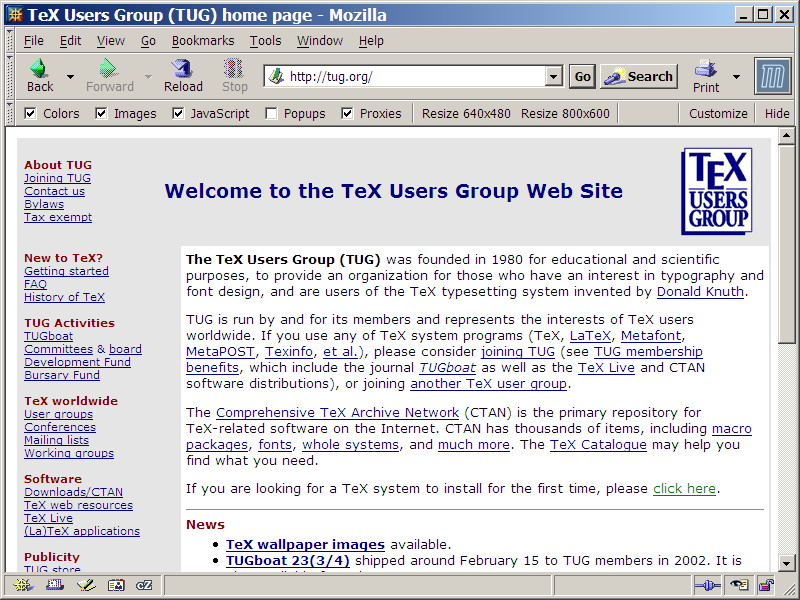
\includegraphics[keepaspectratio,width=\linewidth,height=\halfh]
{images/tugorg.png}

\caption[TeX Users Group web site]{
The web site of the TeX Users Group \parencite{TUG}.
\imgcredit{Screenshot taken by the author of this paper.}
}
\label{fig:TUG}
\end{figure}




\subsection{Installing \protect\LaTeXe}

For information about availability, versions, installation, etc. of
\LaTeXe\ consult the online
\emph{TeX Frequently Asked Questions} \parencite{TeXfaq}.
%
The best way to install \LaTeXe\ under Windows is to get the latest
TeXLive \parencite{texlive} distribution. You can download an ISO
image from CTAN TeXLive \parencite{ctan-texlive}.  Under Windows 10,
you can mount an ISO image by double-clicking, it is no longer
necessary to actually burn the image to a DVD.





\subsection{Installing Extra \protect\LaTeXe Packages}

Depending on the \LaTeXe\ package you install, you may need to install
additional or more recent versions of \LaTeXe\ packages. For example,
this thesis makes use of the \LaTeXe\ \fname{titlesec} package.
%
You can find a list of packages at your local CTAN site \parencite{CTAN}.
To install a package, read the advice at
\url{http://www.ctan.org/installationadvice/}





\subsection{Running \protect\LaTeXe}

When running \LaTeXe\ under Unix, check that the environment variables
are set to something like the values shown here:
\begin{samepage}
\begin{lstlisting}
setenv TEXINPUTS .:~/tex/inputs:./inputs::
setenv BSTINPUTS .:~/tex/inputs::
setenv BIBINPUTS .:~/tex/bib:./bib::
\end{lstlisting}
\end{samepage}


\LaTeXe\ updates certain auxiliary files during translation (for
example with figure numbers or captions) and makes use of them in
subsequent runs. To be absolutely certain that all references are
resolved correctly, run \fname{pdflatex}, \fname{biber},
\fname{pdflatex}, and \fname{pdflatex} in sequence, as shown
below for this thesis:
\begin{samepage}
\begin{lstlisting}
pdflatex thesis
biber thesis
pdflatex thesis
pdflatex thesis
\end{lstlisting}
\end{samepage}




An alternative is to use the \fname{latexmk} perl script:
\begin{samepage}
\begin{lstlisting}
latexmk --pdf thesis
\end{lstlisting}
\end{samepage}


\fname{latexmk} can also be configured using a config file such as
\lstinline|$HOME/.latexmkrc| in the user's home directory: % dummy comment $
\begin{samepage}
\begin{lstlisting}[language=Perl,]
$pdf_mode = 1;  # force use of pdflatex
\end{lstlisting}   % dummy comment $
\end{samepage}


% latexmk
% http://www.ctan.org/pkg/latexmk/
% http://users.phys.psu.edu/~collins/software/latexmk-jcc/
% http://users.phys.psu.edu/~collins/software/latexmk-jcc/latexmk-437.pdf




\subsection{Spell Checking}

GNU Aspell \parencite{Aspell} is a free open source spell checker.  It can
automatically ignore \LaTeXe\ commands. Aspell can either be run from
the command line or integrated into other packages such as Emacs.





\subsection{Integrated Development Environments (IDEs) for \protect\LaTeXe}

Under Windows you might want to use an integrated development
environment (a fancy editor) for \LaTeXe, which have built-in support
for editing \LaTeXe, spell checking, compiling, and so forth.
The IDEs assume that you have a working \LaTeXe installation,
so install \LaTeXe first.
%
The best are Texmaker \parencite{texmaker}, TeXnicCenter
\parencite{TeXnicCenter} (shown in Figure~\ref{fig:TeXnicCenter}), and LEd
\parencite{LEd}, all of which are free. The shareware WinEdt
\parencite{WinEdt} is also very good.


\begin{figure}[tp]
\centering
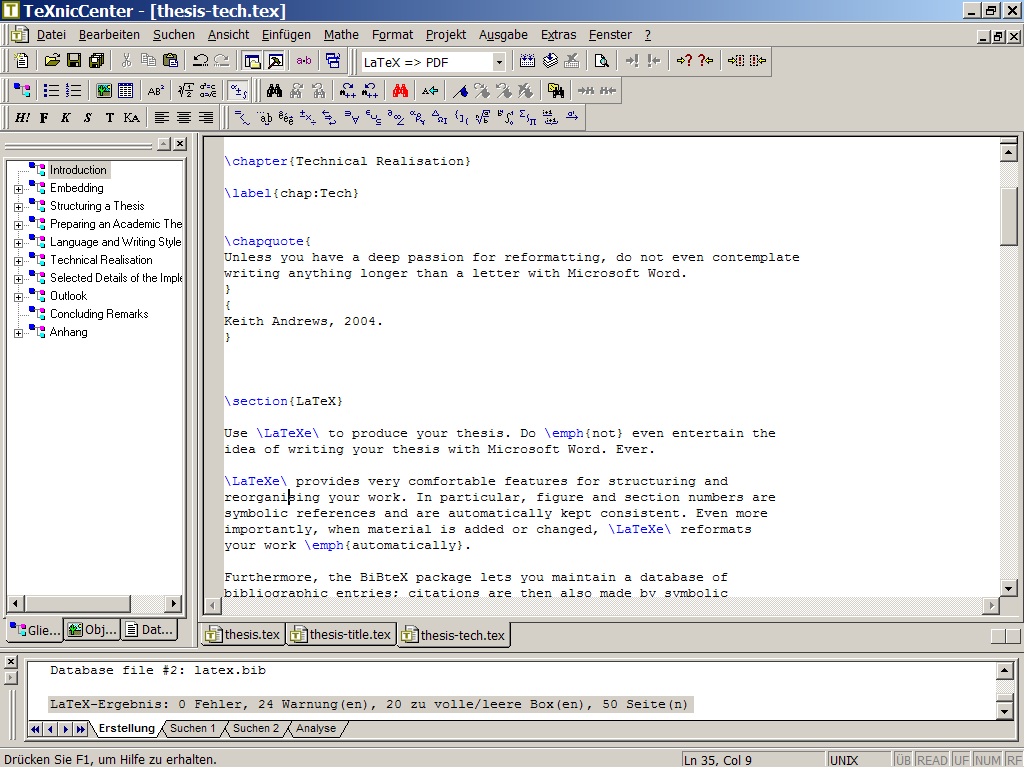
\includegraphics[keepaspectratio,width=\linewidth,height=\halfh]
{images/texnic.png}

\caption[The TeXnicCenter IDE]{
The TeXnicCenter \parencite{TeXnicCenter} integrated development
environment (IDE) for \LaTeXe.
\imgcredit{Screenshot taken by the author of this paper.}
}
\label{fig:TeXnicCenter}
\end{figure}








\section{Including Images}

Use the \fname{graphicx} package to include images:
\begin{samepage}
\begin{lstlisting}
\usepackage{graphicx}
\end{lstlisting}
\end{samepage}



\subsection{Screenshots}

Screenshots should be made using software such as IrfanView or Gimp
and \emph{saved as PNG}. PNG is a lossless image format which
preserves every pixel of the original image. Sometimes, novices save
screenshots as JPEG (\fname{.jpg}), which is an inherently lossy image
format. Screenshots saved as JPEG invariably introduce artefacts such
as smudged lines and text, due to the way that JPEG achieves its high
compression rates.




\subsection{Diagrams}

Diagrams and illustrations should be drawn using a \emph{vector}
graphics editor such as Adobe Illustrator or
Inkscape\parencite{Inkscape}. Archive (and hand-in) the respective source
files (\fname{.ai} or \fname{.svg}). Convert or export the diagram to
vector PDF for inclusion into \LaTeXe.

Vector graphics are based on objects such as lines, circles, polygons,
and text strings and as such are freely scalable without loss of
quality. In contrast, \emph{raster} graphics are based on pixels and
do not scale without loss of quality. Saving diagrams in a raster
format such as PNG, GIF, or JPEG means they cannot be resized without
considerable loss of quality.





\subsection{Graphs and Plots}

Tabular data can be plotted as, say, a line chart or bar chart, using
the free packages \fname{gnuplot} \parencite{gnuplot} or R \parencite{R-Project}.
The plots should be created as SVG (vector graphics), which can then
be touched up, cropped, and converted to PDF using Adobe Illustrator
or Inkscape\parencite{Inkscape}.





\section{Including Listings}

Use the \vname{listings} package to include source code listings.
There are three types of listing:
\begin{itemize}
\item \liintro{Inline}: A small snippet of code can be contained
  within the flow of a paragraph using \lstinline!\lstinline!, for
  example \lstinline|\lstinline!var i:integer;!| produces
  \lstinline!var i:integer;!.

\item \liintro{In-Place Displayed}: An in-place displayed listing is a
  block of code listed at the place where it occurs. Use in-place
  displayed listings for short blocks of source code upto max $n$
  lines (I use $n=4$). Create an in-place displayed listing with the
  \vname{lstlisting} environment, but without using the \vname{float}
  parameter.

\item \liintro{Floating}: A floating listing is a block of code
  treated like other \LaTeXe floats (such as figures or tables). Use
  floating listings for longer blocks of code. \LaTeXe places the
  listing at some point later on. Create a floating listing with the
  \vname{lstlisting} environment, but specify the \vname{float} and
  \vname{caption} parameters. A floating listing is given a number
  (like Listing 2.1) and is listed in the List of Listings.

\end{itemize}

The \vname{listings} package is currently not designed for use with
UTF8 characters. To use UTF8 characters inside listings, you have to
specify the parameter \lstinline!inputencoding=utf8! and 
specify each character inside the \lstinline!literate=! parameter
to the \lstinline!\lstset! command.








\section{Biblatex and Biber}

BibLaTeX \parencite{BibLaTeX} is a companion system to \LaTeXe, which
allows you to manage sets of references in plain text files (called
\fname{.bib} files) and cite references from within your
\LaTeXe\ documents.  Biber \parencite{Biber} is a program which takes
\fname{.bib} files and manages the formatting of citations and of the
bibliography itself. BibLaTeX and Biber have replaced the now obsolete
BibTeX \parencite{BibTeX}.



%\cleardoublepage
%%----------------------------------------------------------------
%
%  File    :  survey-examples.tex
%
%  Author  :  Keith Andrews, IICM, TU Graz, Austria
% 
%  Created :  18 May 2012
% 
%  Changed :  18 May 2012
% 
%----------------------------------------------------------------

\chapter{Selected Examples of Doing Things with \LaTeXe\
(and Test of Extremely
Long Chapter Titles to See How They Work Or Not)
}

\label{chap:SelectedExamples}


This chapter contains some examples of typical \LaTeXe\
usage.





\begin{table}[tp]
\centering
\begin{tabularx}{\linewidth}{|llrX|}
\hline
Name & Type & Rating & Description \\
\hline
Flann O'Brien &
Irish &
***** &
In the centre of town and easy to find for
marauding tourists. Very smooth Guinness.
\\
\hline
The Office &
English &
***** &
Hidden in the narrow streets of the old town.
Erasmus student night every other Wednesday.
\\
\hline
O'Carolans &
Irish &
*** &
In the centre of town in a small side street next to Flann's.
Small, cosy, but hellishly smoky.
\\
\hline
O'Riginal &
pseudo Irish &
 &
Austrian dive pretending to be an Irish pub.
\\
\hline
\end{tabularx}

\caption[Best Pubs in Graz]
{
The best pubs in Graz.
}
\label{tabBestPubs}
\end{table}



\section{Using a Table}

An example of using a table can be seen in Table~\ref{tabBestPubs}.



\section{Using Subfigures}

This example shows how to include vector graphics in the form of PDF
files. It also shows how to use subfigures within a figure.


\begin{figure}[tp]
\centering
\subfloat[%  the % chars remove implicit spacing
An object has been composed to represent an
abstract version of the clock tower in Graz.
Here, the object is in its initial state.
]
{%
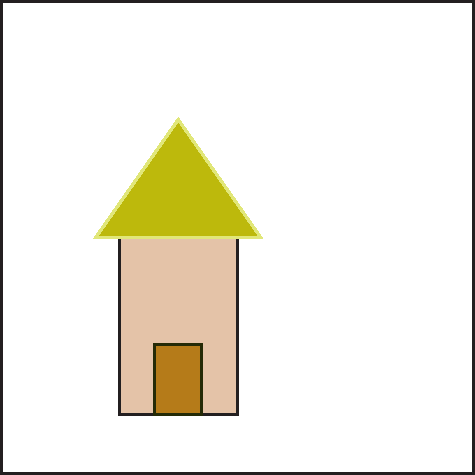
\includegraphics[width=0.45\linewidth]
{diagrams/multi1.pdf}%
\label{figTower1}%
}
\hfill
\subfloat[%
The object has been scaled and rotated, and now resembles
a leaning tower.
]
{%
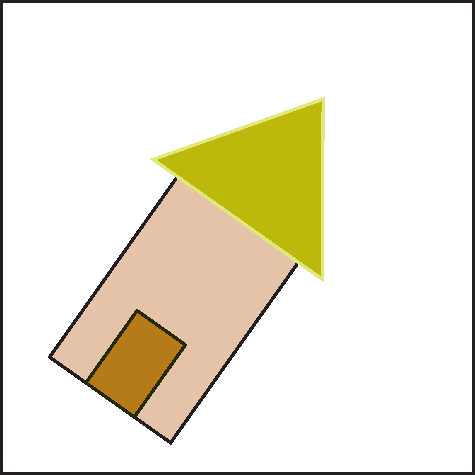
\includegraphics[width=0.45\linewidth]
{diagrams/multi2.pdf}%
\label{figTower2}%
}

\caption[Abstract Clock Towers]
{
The leaning tower of Graz. An abstract model of the clock
tower in Graz leaning over time. \subref{figTower1} shows
the initial state. \subref{figTower2} shows the final state.
\imgcredit{Both images created by the author of this paper.}
}
\label{figWholeFig}
\end{figure}


An example of using the \vname{subfig} package can be seen in
Figure~\ref{figWholeFig}. Figure~\ref{figTower1} shows the polygons
before transformation, while Figure~\ref{figTower2} shows them
afterwards.




\section{Including a Screenshot}


This example shows how to include a screenshot (or other raster
graphic) into a \LaTeXe\ figure.

\begin{figure}[tp]
\centering
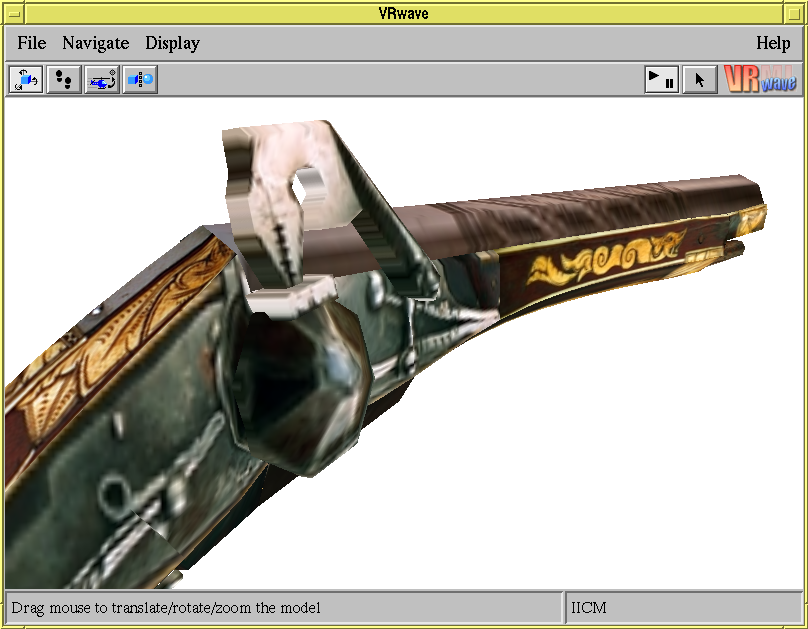
\includegraphics[keepaspectratio,width=\linewidth,height=\halfh]
{images/pist.png}

\caption[VRwave in Flip Mode]
{%
VRwave in Flip mode displaying a textured model of a cavalry pistol
from the world-renowned Zeughaus (armoury) in Graz.
\imgcredit{Image extracted from \textcite[page~81]{Andrews-VRwave}
and used under the terms of the ACM Copyright Policy. \copyrightACM}
}
\label{fig:Pistol}
\end{figure}


An example of how to correctly cite the source when using an image
from someone else. In their 1998 paper, \textcite{Andrews-VRwave} discuss
the VRwave VRML browser. Figure~\ref{fig:Pistol} shows a VRML model of
a cavalry pistol from the Armoury in Graz displayed in the VRwave VRML
browser.





\section{Using Special Characters and Symbols}

You can use many (but not all) of the thousands of characters
available in the UTF-8 \parencites{Wikipedia-UTF8}{Unicode-Charts}
character encoding. For example, the German umlauts (äüö), the German
sharp s (ß), or the yen symbol (¥).

You can also try some of the \approxsym 100 symbols available
in the \vname{textcomp} package, such as the yen symbol (\textyen) and
a circled letter A (\textcircled{A}).



\section{Using Macros to Style Special Names}

Use the \vname{vname}, \vname{cname}, and \vname{fname} macros to
define the style for (say) variable names, class names, and file
names. You can also define your own macros. The is a very long file
name \fname{/usr/data/keith/travel/austria/vienna.txt} to see how they
are broken at a line end. A typical class name is
\cname{HVSInformationPyramidsInputFactory}.




\section{Using Macros as Shorthand}

Sometimes, a macro (new command definition) can be useful to define
the contents of table cells, particularly if these contain images. For
example, Table~\ref{tab:WinIconicLang} uses the macro called
\vname{iibox}, which takes a single parameter, the name of
the particular image.



\begin{table}[tp]

\newcommand{\iibox}[1]{\parbox[c][1cm][c]{1cm}{%
\includegraphics[scale=0.6]{./images/icons/#1}
}}

\begin{center}
\begin{tabular}[t]{|p{7cm}c|}
\hline
\multicolumn{2}{|l|}{\sffamily \bfseries Elementary Symbols}            \\
Document                            & \iibox{win-il-gen-doc}            \\
Assistant                           & \iibox{win-il-gen-ass}            \\
Template                            & \iibox{win-il-gen-tmpl}           \\
\hline
\multicolumn{2}{|l|}{\sffamily \bfseries Document Types}                \\
Text document                       & \iibox{win-il-text-doc}           \\
Spreadsheet document                & \iibox{win-il-spreadsheet-doc}    \\
Presentation document               & \iibox{win-il-presentation-doc}   \\
Database document                   & \iibox{win-il-database-doc}       \\
\hline
\multicolumn{2}{|l|}{\sffamily \bfseries Applications}                  \\
Word                                & \iibox{win-il-word-appl}          \\
Excel                               & \iibox{win-il-xls-appl}           \\
Powerpoint                          & \iibox{win-il-ppt-appl}           \\
Access                              & \iibox{win-il-mdb-appl}           \\
\hline
\multicolumn{2}{|l|}{\sffamily \bfseries Generated Icons}               \\
Word text document                  & \iibox{win-il-word-doc}           \\
Excel spreadsheet document          & \iibox{win-il-xls-doc}            \\
Powerpoint presentation document    & \iibox{win-il-ppt-doc}            \\
Access database document            & \iibox{win-il-mdb-doc}            \\[2ex]
%
Word template                       & \iibox{win-il-word-tmpl}          \\
Powerpoint template                 & \iibox{win-il-ppt-tmpl}           \\
Access template                     & \iibox{win-il-mdb-tmpl}           \\[2ex]
%
Word template assistant             & \iibox{win-il-word-ass}           \\
Powerpoint template assistant       & \iibox{win-il-ppt-ass}            \\
Access template assistant           & \iibox{win-il-mdb-ass}            \\[2ex]
%
\hline
\end{tabular}
\end{center}

\caption[Iconic language for Windows NT 4.0 documents]
{
Iconic language for Windows NT 4.0 documents.
\imgcredit{The icons are screenshots, captured and then
enlarged by the author of this paper.}
}
\label{tab:WinIconicLang}
\end{table}






\section{Using Floating Listings}

\begin{samepage}
\begin{lstlisting}[%
  float=tp,
  aboveskip=\floatsep,
  belowskip=\floatsep,
  xleftmargin=0cm,              % no extra margins for floats
  xrightmargin=0cm,             % no extra margins for floats
  language=HTML,
  basicstyle=\footnotesize\ttfamily,
  frame=shadowbox,
  numbers=left,
  label=list:HTML5Boilerplate,
  caption={[HTML5 Boilerplate Code]%
Some HTML5 boilerplate code, illustrating the typical structure
of a HTML5 web page.
},
]
<!DOCTYPE html>
<html xmlns="http://www.w3.org/1999/xhtml" lang="en" xml:lang="en">

<head>
<meta charset="UTF-8"/>
<meta name="viewport" content="width=device-width, initial-scale=1"/>
<link rel="stylesheet" href="./inm.css"/>

<title>Keith Andrews Web Page</title>
</head>

<body>

<header>
<img src="images/kalogo.svg" alt="KA Logo"/>
Keith Andrews Design
</header>

<h1>Keith Andrews</h1>

<p>
Keith lives in <a href="http://graz.at/">Graz</a>.
</p>

<p>
<img src="images/keith-s.jpg"
  alt="Photo of Keith Andrews"/>
</p>

<p>
Three desirable attributes:
</p>
<ol>
<li>cheap</li>
<li>fast</li>
<li>good</li>
</ol>
<p>
Choose any two.
</p>

<p>
<abbr title="Extensible HyperText Markup Language">XHTML</abbr>
is cool.
</p>

<table>
<tbody>
<tr><th>Beer</th><th>Price €</th></tr>
<tr><td>Puntigamer</td><td>2,60</td></tr>
<tr><td>Gösser</td><td>2,60</td></tr>
<tr><td>Guinness</td><td>4,35</td></tr>
</tbody>
</table>

<footer>
Copyright © Keith Andrews 2019.
</footer>

</body>
</html>
\end{lstlisting}
\end{samepage}

Listing~\ref{list:HTML5Boilerplate} is floating. A floating listing is
a block of code treated like other \LaTeXe floats (such as figures or
tables). Use floating listings for longer blocks of code.
A floating listing is given a number and can be referred to
explicitly, like Listing~\ref{list:HTML5Boilerplate}. It can be given
a caption and short caption, and is listed in the List of Listings.





\section{Using Non-Floating Diplayed Listings}

The listing below shows some CSS:
\begin{samepage}
\begin{lstlisting}[%
  language=CSS,
]
body { color: black; background-color: silver; }
img { border: none; }
h1,h2 { font-family: Verdana, sans-serif; }
\end{lstlisting}
\end{samepage}
It is displayed (i.e. indented as a block) in-place, but is not
floating. It cannot be referred to by number and is not listed in the
List of Listings. As a rule of thumb, if listings have five or more
lines, make them floating.





\section{Using Inline Listings}

Inline listings are used for very short snippets of code embedded
within the flow of a paragraph. For example,
\lstinline|\lstinline!var i:integer;!|
produces
\lstinline!var i:integer;!, which can now be discussed further.
Do not break an inline listing over multiple lines (EOL).




\section{Using Lists}

A list should always be introduced by a sentence
which ends with a colon.
%
There are three kinds of standard lists in \LaTeXe:
\begin{itemize}
\item itemize
\item enumerate
\item description
\end{itemize}
% A blank line here would indicate a new (indented) paragraph
An enumerated list has numbered items:
\begin{enumerate}
\item Fast
\item Good
\item Cheap
\end{enumerate}
Choose any two!


A description list has named items with corresponding
definitions or descriptions:
\begin{description}
\item[Short] Each item has a label (name) and its description.

\item[Rather longer label] By default, if the description text
  is rather long, it will warp around to the following lines.
\end{description}





%\cleardoublepage
%%----------------------------------------------------------------
%
%  File    :  survey-concl.tex
%
%  Author  :  Keith Andrews, IICM, TU Graz, Austria
% 
%  Created :  27 May 1993
% 
%  Changed :  16 Nov 2010
% 
%----------------------------------------------------------------


\chapter{Concluding Remarks}

\label{chap:Concl}



At the end of your survey, give a clear recommendation
as to which approach or tool to use in which situation.





\cleardoublepage
% for now, switch to language english
% hack to force unix date for biblio, biblatex 3.11
\begin{otherlanguage}{english}
\printbibliography[heading=bibintoc]
\end{otherlanguage}


\end{document} 


